\documentclass[10 pt]{beamer}
\usetheme{Madrid}
\usepackage[utf8]{inputenc}
\usepackage{xspace}
\usepackage{graphicx,graphics} 
\usepackage{color}
\usepackage{amsmath}
\usepackage{amsfonts}
\usepackage{amssymb}
\usepackage{amsthm}
\usepackage{tabularx}
\usepackage{algorithm}
\usepackage{algorithmic}
\usepackage{longtable}
\usepackage{complexity}
\usepackage{tkz-graph}
\usepackage{float}
\usepackage{multicol}
\usepackage{setspace}
\usepackage[absolute,overlay]{textpos}
\beamertemplatenavigationsymbolsempty
\graphicspath{{fig/}}

\tikzset{
  LabelStyle/.style = { rectangle, rounded corners, draw,
                       font = \bfseries },
  EdgeStyle/.append style = {-} }
\title{Deterministic scheduling of periodic datagrams for low latency in 5G and beyond}

\author{{\bf Maël~Guiraud}}

\AtBeginSection[]{
  \begin{frame}
  \vfill
  \centering
  \begin{beamercolorbox}[sep=8pt,center,shadow=true,rounded=true]{title}
    \usebeamerfont{title}\insertsectionhead\par%
  \end{beamercolorbox}
  \vfill
  \end{frame}
}

\institute[Nokia Bell Labs, DAVID-UVSQ] 
{
  Nokia Bell Labs France - DAVID, Universit\'e de Versailles Saint Quentin
   \\
}

\subject{Theoretical Computer Science}
\newcommand{\todo}[1]{{\color{red} TODO: {#1}}}


\begin{document}


\begin{frame}

  \titlepage
  \centering
  
\includegraphics [width=25mm]{logon.png} \hspace{1cm} 
\includegraphics [width=17.5mm]{logod.png} \\
\end{frame}




\section{Introduction }
\subsection{Context }


\begin{frame}{5G Context}


  \centering
  
  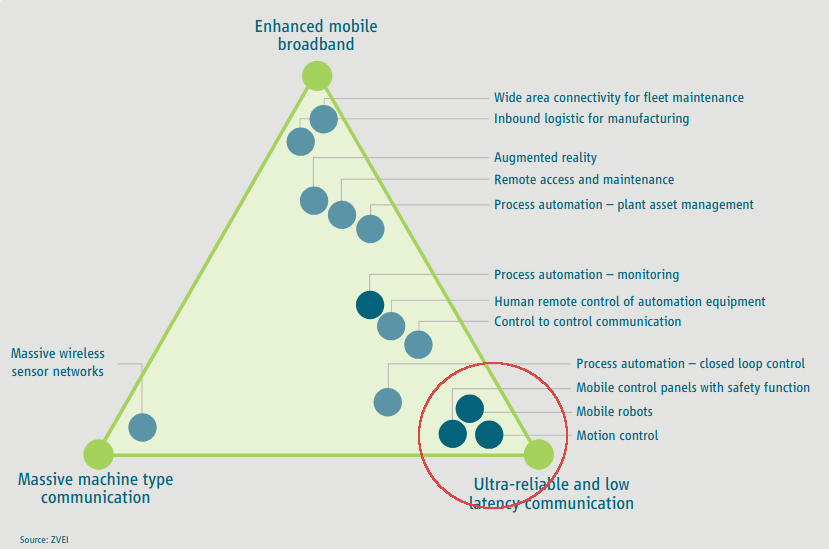
\includegraphics[scale=0.4]{usecases.png}
  

\end{frame}
\begin{frame}{Use cases}


  \centering
  
  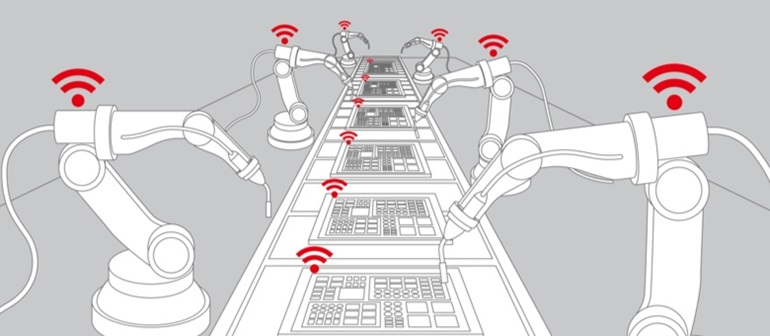
\includegraphics[scale=0.4]{ind40.jpg}

  Industry 4.0

\end{frame}
\begin{frame}{Use cases}


  \centering
  
  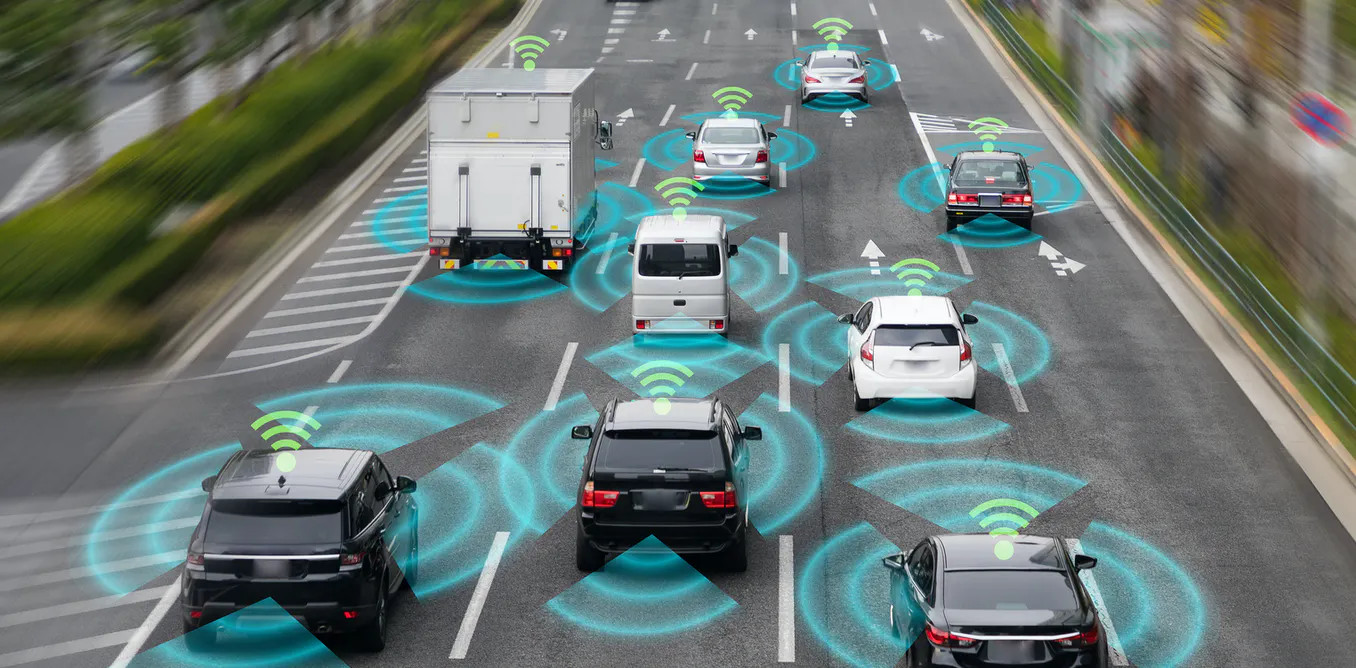
\includegraphics[scale=0.25]{vehicle.jpg}

  Autonomous Vehicle

\end{frame}

\begin{frame}{A Radio Antenna}
\begin{center}
  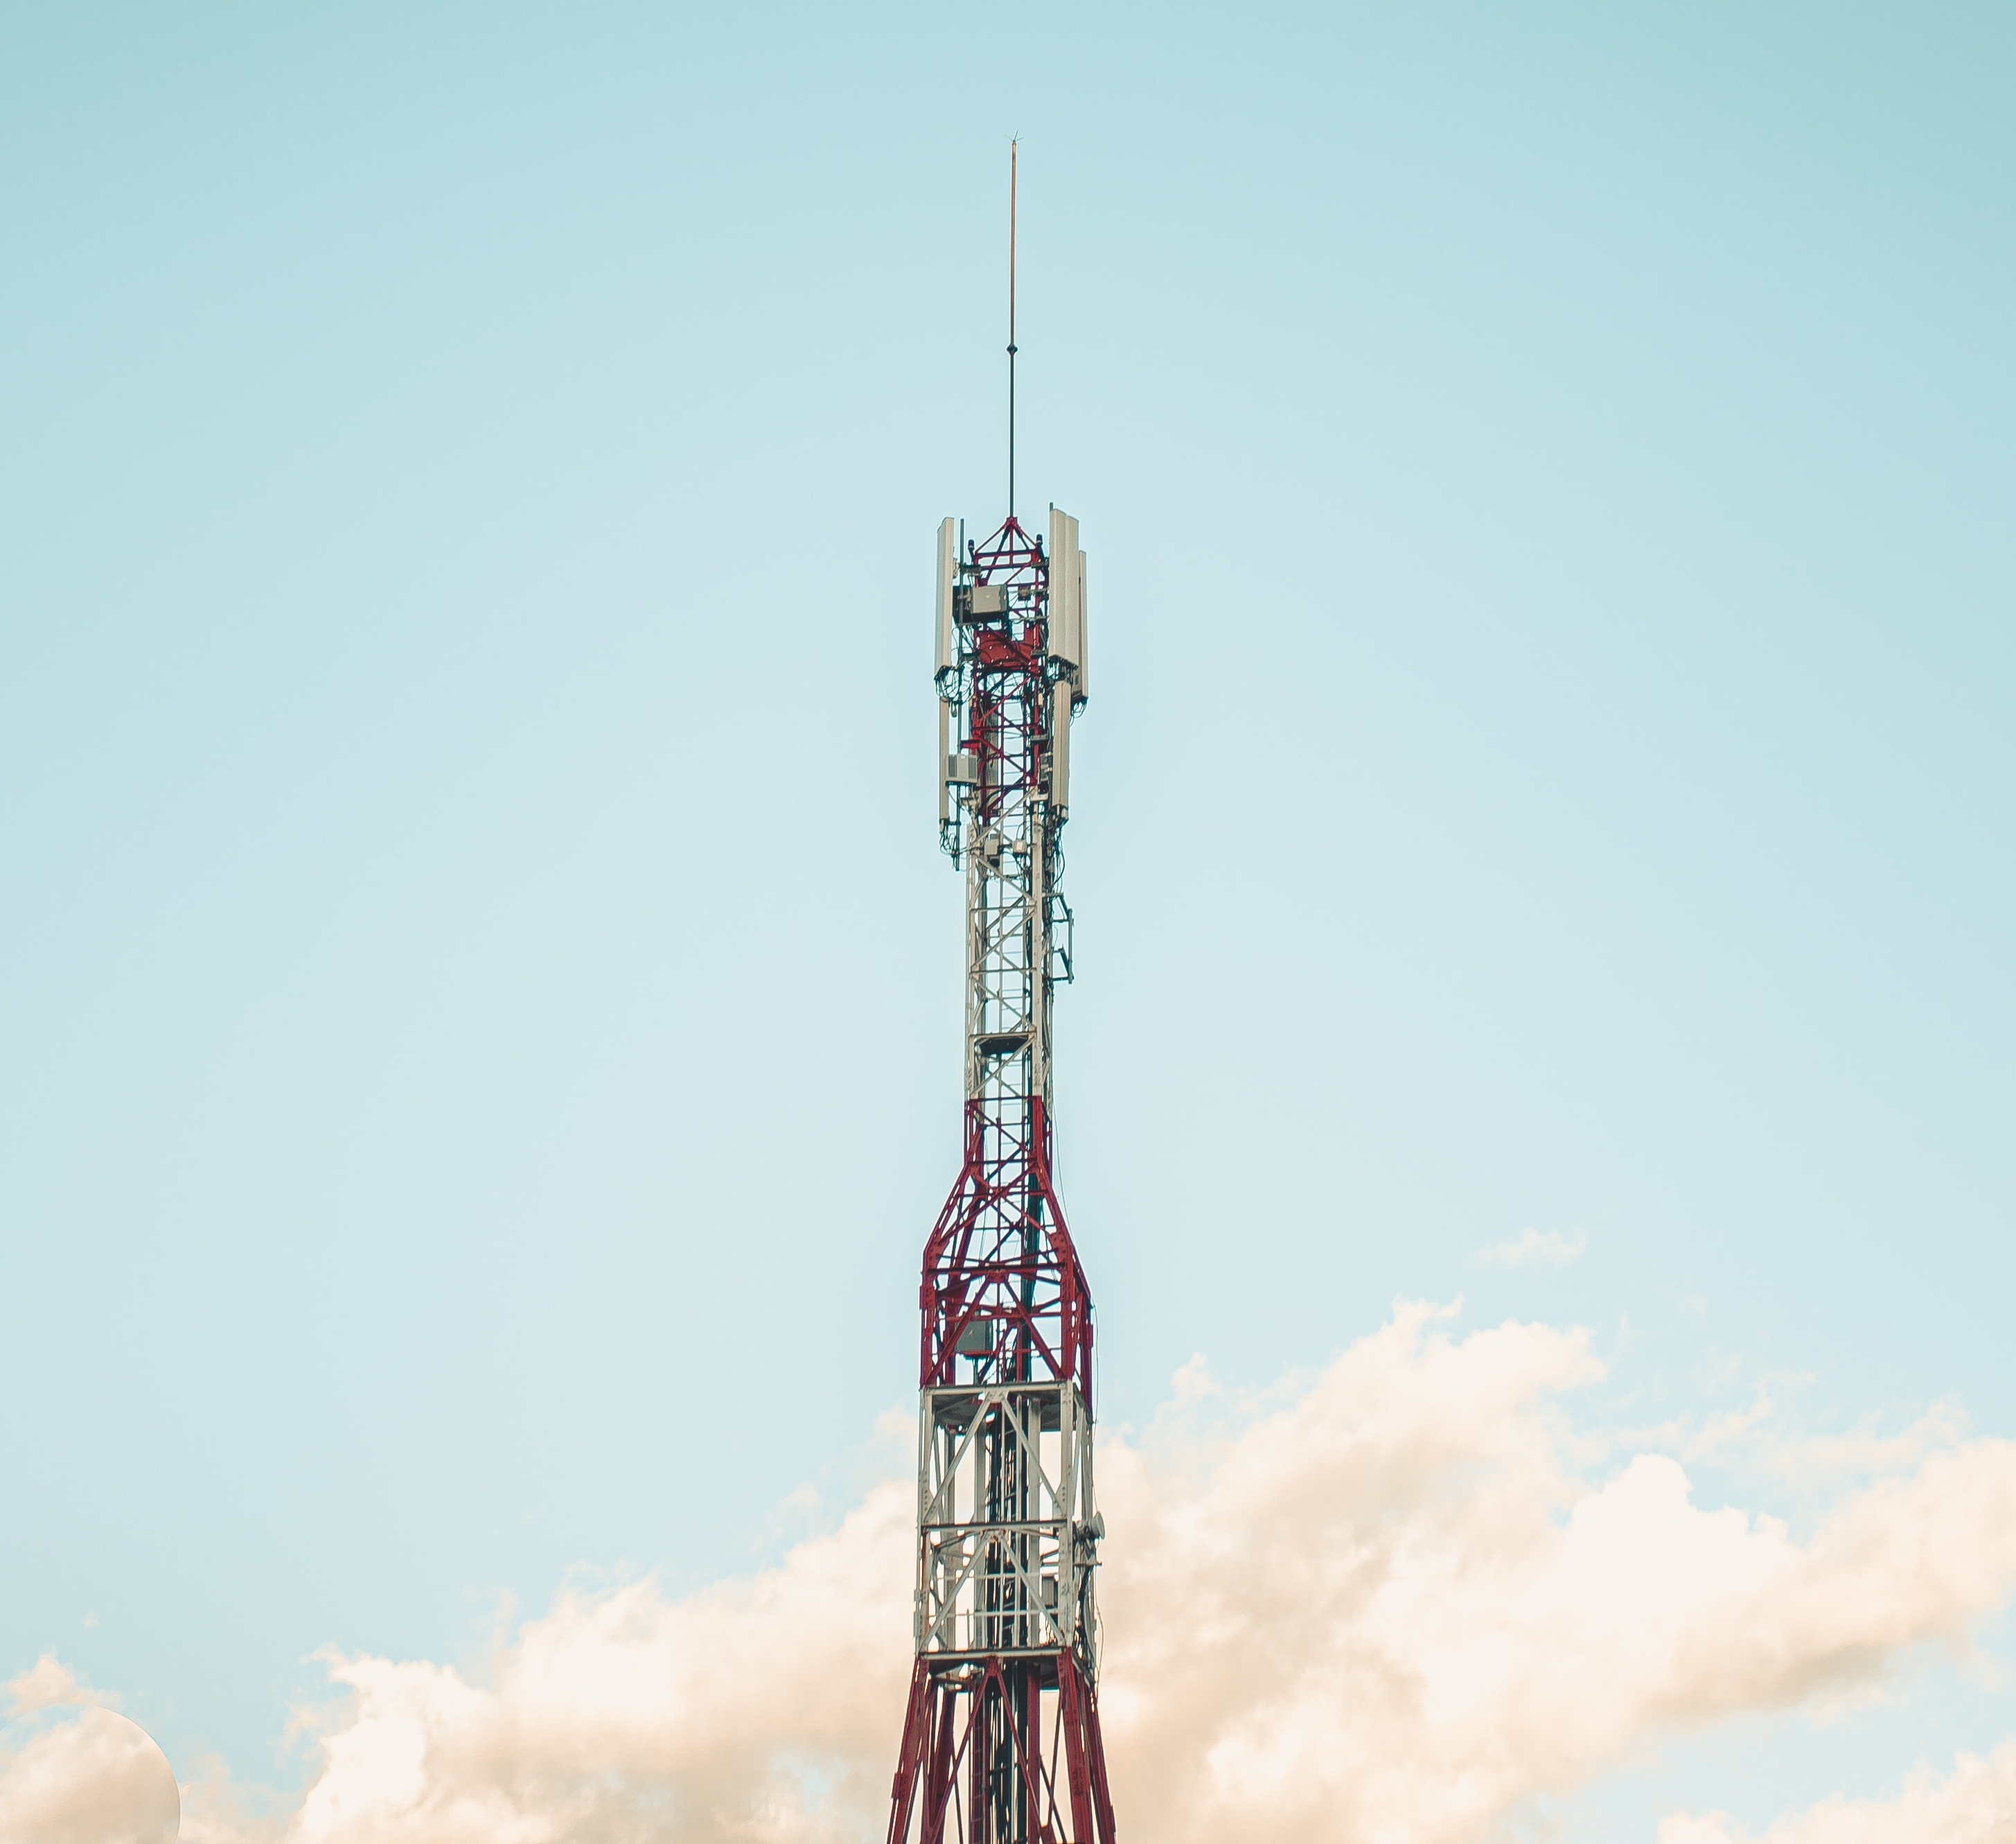
\includegraphics [width=\textwidth]{radio.jpg} 
\end{center}

\end{frame}
\begin{frame}{A Radio Antenna}
\begin{center}
  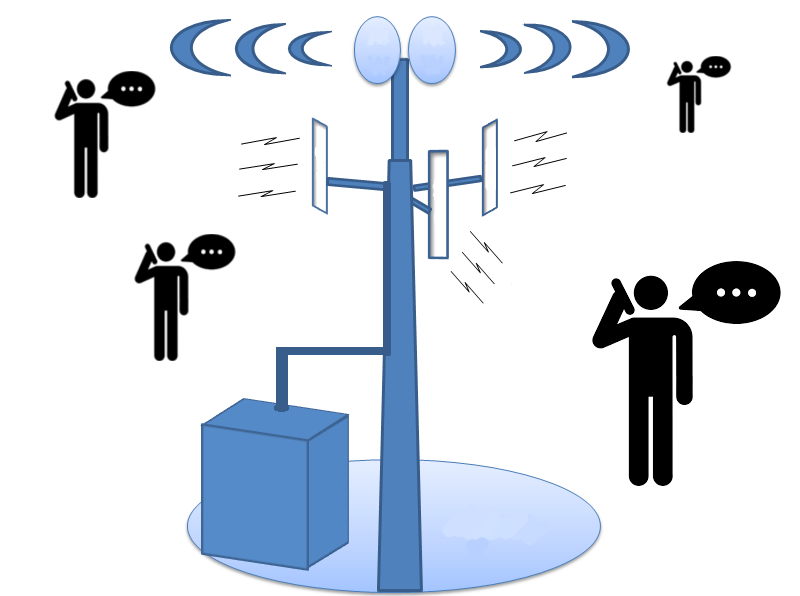
\includegraphics[scale=0.3]{btsppl.png}

\end{center}

\end{frame}

\begin{frame}{Radio Access Network}

\scalebox{0.4}{

\begin{tikzpicture}
  \SetGraphUnit{5}
    \tikzset{
  EdgeStyle/.append style = {->} }
   \tikzstyle{VertexStyle}=[shape = circle, draw, minimum size = 30pt]
 

  \node (p1) at (0,4) {
\includegraphics[width = 1cm]{phone.png}};
 
  \node (p2) at (0,2) {
\includegraphics[width = 1cm]{phone.png}};

  \node (p3) at (0,0) {
\includegraphics[width = 1cm]{phone.png}};
  
   \node (r1) at (4,2) {
\includegraphics[width = 1cm]{rrh.png}};


 
\path (p1) edge [<->,color=red]  (r1);
\path (p2) edge [<->]  (r1);
\path (p3) edge [<->]  (r1);

\end{tikzpicture}
}


\end{frame}
\begin{frame}{Radio Access Network}

\scalebox{0.4}{

\begin{tikzpicture}
  \SetGraphUnit{5}
    \tikzset{
  EdgeStyle/.append style = {->} }
   \tikzstyle{VertexStyle}=[shape = circle, draw, minimum size = 30pt]
 

  \node (p1) at (0,4) {
\includegraphics[width = 1cm]{phone.png}};
 
  \node (p2) at (0,2) {
\includegraphics[width = 1cm]{phone.png}};

  \node (p3) at (0,0) {
\includegraphics[width = 1cm]{phone.png}};
  
   \node (r1) at (4,2) {
\includegraphics[width = 1cm]{rrh.png}};


 
\path (p1) edge [<->,color=red]  (r1);
\path (p2) edge [<->]  (r1);
\path (p3) edge [<->]  (r1);
\node at (3, 4) {RAN};
\end{tikzpicture}
}


\end{frame}

\begin{frame}{Aggregation network}
\scalebox{0.4}{

\begin{tikzpicture}
  \SetGraphUnit{5}
    \tikzset{
  EdgeStyle/.append style = {->} }
   \tikzstyle{VertexStyle}=[shape = circle, draw, minimum size = 30pt]
 

  \node (p1) at (0,4) {
\includegraphics[width = 1cm]{phone.png}};
 
  \node (p2) at (0,2) {
\includegraphics[width = 1cm]{phone.png}};

  \node (p3) at (0,0) {
\includegraphics[width = 1cm]{phone.png}};
  
 \node (a1) at (7,1) {
\includegraphics[width = 1cm]{switch.png}};
 \node (a2) at (7,3) {
\includegraphics[width = 1cm]{switch.png}};
 \node (a3) at (9,1) {
\includegraphics[width = 1cm]{switch.png}};
 \node (a4) at (9,3) {
\includegraphics[width = 1cm]{switch.png}};

  
   \node (r1) at (4,2) {
\includegraphics[width = 1cm]{rrh.png}};

   

 
\path (p1) edge [<->,color=red]  (r1);
\path (p2) edge [<->]  (r1);
\path (p3) edge [<->]  (r1);

\path (r1) edge [<->,color=red]  (a1);
\path (r1) edge [<->]  (a2);

\path (a1) edge [<->]  (a2);
\path (a3) edge [<->]  (a2);
\path (a4) edge [<->]  (a2);
\path (a3) edge [<->]  (a4);
\path (a3) edge [<->]  (a1);
\path (a4) edge [<->,color=red]  (a1);
\node at (3, 4) {RAN};


\end{tikzpicture}
}

\end{frame}


\begin{frame}{Aggregation network}
\scalebox{0.4}{

\begin{tikzpicture}
  \SetGraphUnit{5}
    \tikzset{
  EdgeStyle/.append style = {->} }
   \tikzstyle{VertexStyle}=[shape = circle, draw, minimum size = 30pt]
 

  \node (p1) at (0,4) {
\includegraphics[width = 1cm]{phone.png}};
 
  \node (p2) at (0,2) {
\includegraphics[width = 1cm]{phone.png}};

  \node (p3) at (0,0) {
\includegraphics[width = 1cm]{phone.png}};
  
 \node (a1) at (7,1) {
\includegraphics[width = 1cm]{switch.png}};
 \node (a2) at (7,3) {
\includegraphics[width = 1cm]{switch.png}};
 \node (a3) at (9,1) {
\includegraphics[width = 1cm]{switch.png}};
 \node (a4) at (9,3) {
\includegraphics[width = 1cm]{switch.png}};

  
   \node (r1) at (4,2) {
\includegraphics[width = 1cm]{rrh.png}};

   

 
\path (p1) edge [<->,color=red]  (r1);
\path (p2) edge [<->]  (r1);
\path (p3) edge [<->]  (r1);

\path (r1) edge [<->,color=red]  (a1);
\path (r1) edge [<->]  (a2);

\path (a1) edge [<->]  (a2);
\path (a3) edge [<->]  (a2);
\path (a4) edge [<->]  (a2);
\path (a3) edge [<->]  (a4);
\path (a3) edge [<->]  (a1);
\path (a4) edge [<->,color=red]  (a1);


\node at (3, 4) {RAN};
\node at (8, 4) {Aggregation};

\end{tikzpicture}
}

\end{frame}



\begin{frame}{An end-to-end communication between two terminals}
\scalebox{0.4}{

\begin{tikzpicture}
  \SetGraphUnit{5}
    \tikzset{
  EdgeStyle/.append style = {->} }
   \tikzstyle{VertexStyle}=[shape = circle, draw, minimum size = 30pt]
 

  \node (p1) at (0,4) {
\includegraphics[width = 1cm]{phone.png}};
 
  \node (p2) at (0,2) {
\includegraphics[width = 1cm]{phone.png}};

  \node (p3) at (0,0) {
\includegraphics[width = 1cm]{phone.png}};
  
 \node (a1) at (7,1) {
\includegraphics[width = 1cm]{switch.png}};
 \node (a2) at (7,3) {
\includegraphics[width = 1cm]{switch.png}};
 \node (a3) at (9,1) {
\includegraphics[width = 1cm]{switch.png}};
 \node (a4) at (9,3) {
\includegraphics[width = 1cm]{switch.png}};

 \node (c1) at (12,3) {
\includegraphics[width = 1cm]{switch.png}};
 \node (c2) at (12,5) {
\includegraphics[width = 1cm]{switch.png}};
 \node (c3) at (14,3) {
\includegraphics[width = 1cm]{switch.png}};
 \node (c4) at (14,5) {
\includegraphics[width = 1cm]{switch.png}};

 \node (a5) at (17,1) {
\includegraphics[width = 1cm]{switch.png}};
 \node (a6) at (17,3) {
\includegraphics[width = 1cm]{switch.png}};
 \node (a7) at (19,1) {
\includegraphics[width = 1cm]{switch.png}};
 \node (a8) at (19,3) {
\includegraphics[width = 1cm]{switch.png}};


 \node (p4) at (26,4) {
\includegraphics[width = 1cm]{phone.png}};
 
  \node (p5) at (26,2) {
\includegraphics[width = 1cm]{phone.png}};

  \node (p6) at (26,0) {
\includegraphics[width = 1cm]{phone.png}};
  
   \node (r1) at (4,2) {
\includegraphics[width = 1cm]{rrh.png}};
   \node (r2) at (22,2) {\includegraphics[width = 1cm]{rrh.png}};
   

 
\path (p1) edge [<->,color=red]  (r1);
\path (p2) edge [<->]  (r1);
\path (p3) edge [<->]  (r1);

\path (r1) edge [<->,color=red]  (a1);
\path (r1) edge [<->]  (a2);

\path (a1) edge [<->]  (a2);
\path (a3) edge [<->]  (a2);
\path (a4) edge [<->]  (a2);
\path (a3) edge [<->]  (a4);
\path (a3) edge [<->]  (a1);
\path (a4) edge [<->,color=red]  (a1);


\path (c1) edge [<->]  (c2);
\path (c3) edge [<->]  (c2);
\path (c4) edge [<->]  (c2);
\path (c3) edge [<->]  (c4);
\path (c3) edge [<->]  (c1);
\path (c4) edge [<->,color=red]  (c1);


\path (a5) edge [<->]  (a6);
\path (a7) edge [<->]  (a6);
\path (a8) edge [<->,color=red]  (a6);
\path (a7) edge [<->]  (a8);
\path (a7) edge [<->]  (a5);
\path (a8) edge [<->]  (a5);

 
\path (p4) edge [<->]  (r2);
\path (p5) edge [<->,color=red]  (r2);
\path (p6) edge [<->]  (r2);


\path (a4) edge [<->]  (c2);
\path (a3) edge [<->]  (c1);
\path (a3) edge [<->]  (c2);
\path (a4) edge [<->,color=red]  (c1);


\path (a6) edge [<->,color=red]  (c4);
\path (a5) edge [<->]  (c3);
\path (a5) edge [<->]  (c4);
\path (a6) edge [<->]  (c3);

\path (r2) edge [<->,color=red]  (a8);
\path (r2) edge [<->]  (a7);
\draw[dashed] (-1,-1) rectangle  (10,7);
\node at (3, 4) {RAN};
\node at (8, 4) {Aggregation};

\draw[dashed] (16,-1) rectangle  (27,7);
\node at (23, 4) {RAN};
\node at (18, 4) {Aggregation};

\draw[dashed] (11,2) rectangle  (15,7);
\node at (13, 6.5) {\huge Core};

\end{tikzpicture}
}

\end{frame}



\begin{frame}{What does Cloud-RAN means?}
  \centering
  \includegraphics[scale=0.2]{cloudbts.png}\\
  \includegraphics[scale=0.175]{BBURRH.png}
  
   RU=RRH, Distributed/Centralized Unit=BBU
\end{frame}



\begin{frame}{Cloud-RAN}
  \centering
  \includegraphics[scale=0.3]{CRAN}\\
  \vspace{0.5cm}
  \pause
  C-RAN aims to mutualize the computation ressources.
  
  \pause

  The latency is constrained by protocol.
  
  
\end{frame}


\begin{frame}{Problematic}
  \centering
  
  \begin{center}
  \includegraphics [width=6cm]{modelstar} 
\end{center}

 \begin{multicols}{2}
Statistical multiplexing:


\begin{itemize}
\item Buffering inducing additional latency
\item Average guarantee on Latency
\end{itemize}
\vspace{2cm}

C-RAN specifications:
 \begin{itemize}
\item $100\%$ of the packets under a given latency.
\item Minimize latency means an higher area cover.
\end{itemize}

\end{multicols}

\end{frame}


\subsection{Model, problems}
 
\begin{frame}{Model: The routed network}
\begin{center}
  \includegraphics [width=9cm]{1routealler} 
\end{center}

\begin{itemize}
\item Network $\rightarrow$ Weighted Directed Acyclic Multigraph
\item  Discrete time model: Physical Delay of a link $\rightarrow$ Weight of the arcs (tics).
\item  Only the contention points are represented in the graph
\end{itemize}

\begin{center}
\scalebox{0.6}{

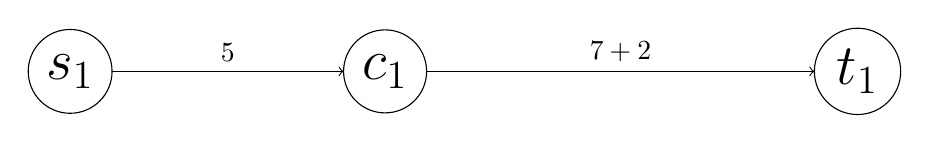
\begin{tikzpicture}
  \SetGraphUnit{5}
    \tikzset{
  EdgeStyle/.append style = {->} }
   \tikzstyle{VertexStyle}=[shape = circle, draw, minimum size = 30pt]
   \renewcommand{\VertexLightFillColor}{orange}
  \Vertex[x=0,y=0, L = {\huge $s_1$}]{s1};

\Vertex[x=10,y=0, L = {\huge $t_1$}]{t1};

  \Vertex[x=4,y=0, L = {\huge $c_1$}]{c1}
  
 %\SetVertexNoLabel
  %\Vertex[x=4,y=2]{n1}

 % \Edge[label = $5$](s1)(c1)
 % \Edge[label = $7 + 2$](c1)(t1)
  \path (s1) edge [->] node[anchor=south]{$5$} (c1);
\path (c1) edge [->] node[anchor=south]{$7+2$} (t1);

 


\end{tikzpicture}
}
  \end{center}


 \end{frame}
 
\begin{frame}{Model: The routed network}
Both ways: from RRH to BBU (forward) then from BBU to RRH (backward)
 \begin{center}
  \includegraphics [width=9cm]{1routeretour} 
\end{center}


\begin{center}
\scalebox{0.6}{

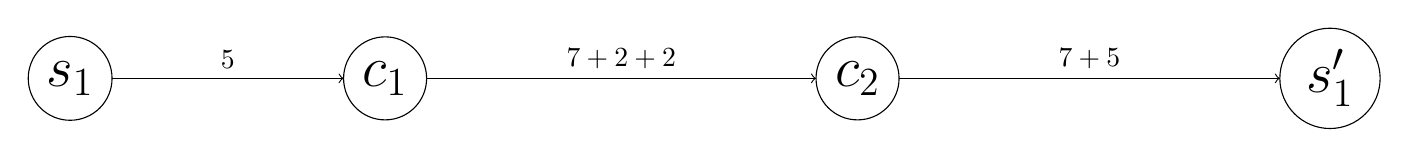
\begin{tikzpicture}
  \SetGraphUnit{5}
    \tikzset{
  EdgeStyle/.append style = {->} }
   \tikzstyle{VertexStyle}=[shape = circle, draw, minimum size = 30pt]
   \renewcommand{\VertexLightFillColor}{orange}
  \Vertex[x=0,y=0, L = {\huge $s_1$}]{s1};
\Vertex[x=16,y=0, L = {\huge $s_1'$}]{s1p};
\Vertex[x=10,y=0, L = {\huge $c_2$}]{c2};

  \Vertex[x=4,y=0, L = {\huge $c_1$}]{c1}
  
 %\SetVertexNoLabel
  %\Vertex[x=4,y=2]{n1}

  %\Edge[label = $5$](s1)(c1)
 % \Edge[label = $7 + 2+2$](c1)(c2)
 % \Edge[label = $7 + 2+2$](c1)(c2)
%\Edge[label = $7 + 5$](c2)(s1p)
 
\path (s1) edge [->] node[anchor=south]{$5$} (c1);
\path (c1) edge [->] node[anchor=south]{$7+2+2$} (c2);
\path (c2) edge [->] node[anchor=south]{$7+5$} (s1p);


\end{tikzpicture}
}
\end{center}
\end{frame}

\begin{frame}{Model: The routed network}

 \begin{center}
  \includegraphics [width=7.5cm]{starfronthaul} 
\end{center}


\begin{center}
\scalebox{0.6}{

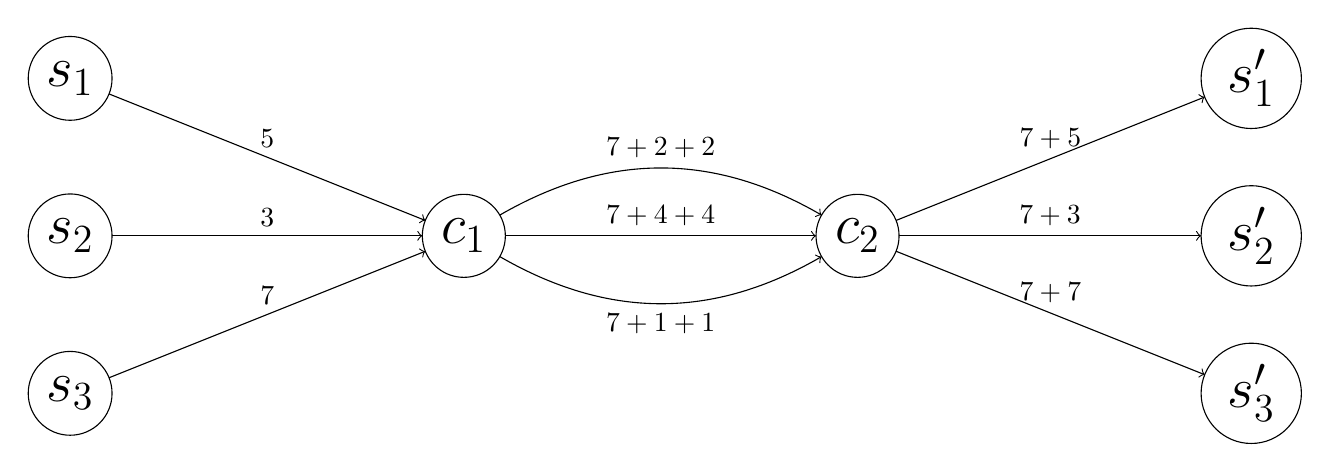
\begin{tikzpicture}
  \SetGraphUnit{5}
    \tikzset{
  EdgeStyle/.append style = {->} }
   \tikzstyle{VertexStyle}=[shape = circle, draw, minimum size = 30pt]
   \renewcommand{\VertexLightFillColor}{orange}
  \Vertex[x=0,y=4, L = {\huge $s_1$}]{s1};
  \Vertex[x=0,y=2, L = {\huge $s_2$}]{s2};
\Vertex[x=0,y=0, L = {\huge $s_3$}]{s3};
\Vertex[x=15,y=4, L = {\huge $s_1'$}]{s1p};
\Vertex[x=15,y=2, L = {\huge $s_2'$}]{s2p};
\Vertex[x=15,y=0, L = {\huge $s_3'$}]{s3p};
\Vertex[x=10,y=2, L = {\huge $c_2$}]{c2};

  \Vertex[x=5,y=2, L = {\huge $c_1$}]{c1}
  
 %\SetVertexNoLabel
  %\Vertex[x=4,y=2]{n1}

  %\Edge[label = $5$](s1)(c1)
  %\Edge[label = $7 + 4+4$](c1)(c2)
  %\Edge[label = $3$](s2)(c1)
   %\Edge[label = $7$](s3)(c1)
  %  \Edge[label = $7+3$](c2)(s2p)
 %  \Edge[label = $7+7$](c2)(s3p)
%\Edge[label = $7 + 5$](c2)(s1p)
\path (s1) edge [->] node[anchor=south]{$5$} (c1);

\path (s2) edge [->] node[anchor=south]{$3$} (c1);
\path (s3) edge [->] node[anchor=south]{$7$} (c1);
\path (c2) edge [->] node[anchor=south]{$7+3$} (s2p);
\path (c2) edge [->] node[anchor=south]{$7+7$} (s3p);

\path (c2) edge [->] node[anchor=south]{$7+5$} (s1p);

\path (c1) edge [->] node[anchor=south]{$7+4+4$} (c2);

\path (c1) edge [->,bend left=30] node[anchor=south]{$7+2+2$} (c2);
\path (c1) edge [->,bend right=30] node[anchor=north]{$7+1+1$} (c2);

  %\draw[->,line width=0.5pt] (5,2.51) parabola bend (7.5,3.5) (10,2.51);
 %\draw[->,line width=0.5pt] (5,1.49) parabola bend (7.5,0.5) (10,1.49);
 

\end{tikzpicture}
}

\end{center}
\end{frame}
  \begin{frame}{Model: The communication process}
 
 \begin{center}
\scalebox{0.3}{

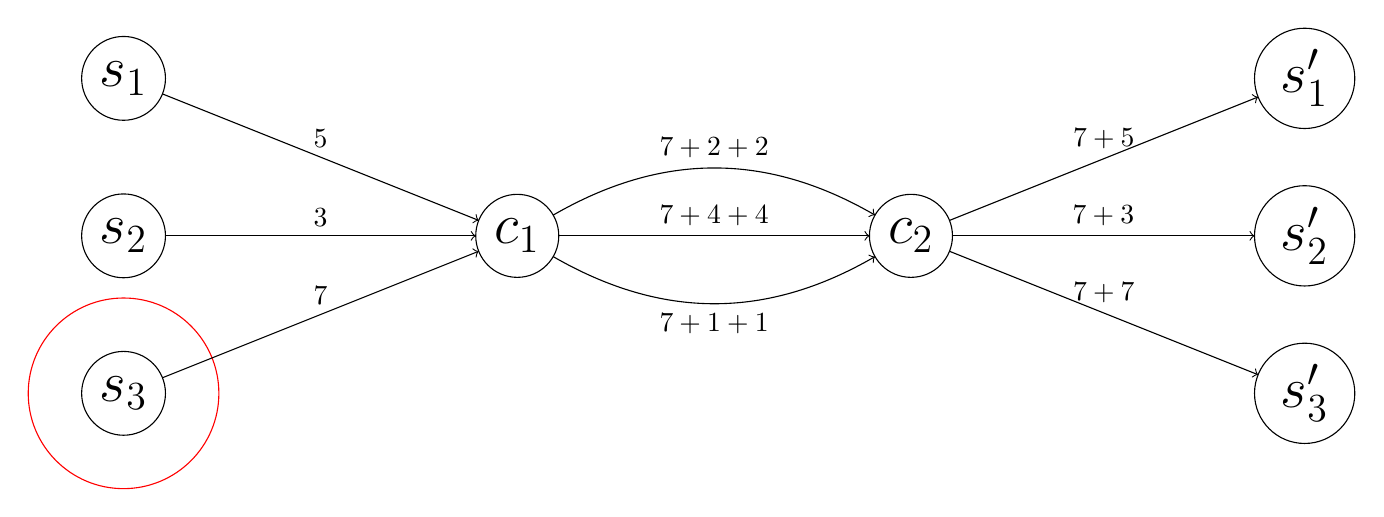
\begin{tikzpicture}
  \SetGraphUnit{5}
    \tikzset{
  EdgeStyle/.append style = {->} }
   \tikzstyle{VertexStyle}=[shape = circle, draw, minimum size = 30pt]
   \renewcommand{\VertexLightFillColor}{orange}
  \Vertex[x=0,y=4, L = {\huge $s_1$}]{s1};
  \Vertex[x=0,y=2, L = {\huge $s_2$}]{s2};
\Vertex[x=0,y=0, L = {\huge $s_3$}]{s3};
\Vertex[x=15,y=4, L = {\huge $s_1'$}]{s1p};
\Vertex[x=15,y=2, L = {\huge $s_2'$}]{s2p};
\Vertex[x=15,y=0, L = {\huge $s_3'$}]{s3p};
\draw[red] (0,0) circle (8ex);
\Vertex[x=10,y=2, L = {\huge $c_2$}]{c2};

  \Vertex[x=5,y=2, L = {\huge $c_1$}]{c1}
  
 %\SetVertexNoLabel
  %\Vertex[x=4,y=2]{n1}

  %\Edge[label = $5$](s1)(c1)
  %\Edge[label = $7 + 4+4$](c1)(c2)
  %\Edge[label = $3$](s2)(c1)
   %\Edge[label = $7$](s3)(c1)
  %  \Edge[label = $7+3$](c2)(s2p)
 %  \Edge[label = $7+7$](c2)(s3p)
%\Edge[label = $7 + 5$](c2)(s1p)
\path (s1) edge [->] node[anchor=south]{$5$} (c1);

\path (s2) edge [->] node[anchor=south]{$3$} (c1);
\path (s3) edge [->] node[anchor=south]{$7$} (c1);
\path (c2) edge [->] node[anchor=south]{$7+3$} (s2p);
\path (c2) edge [->] node[anchor=south]{$7+7$} (s3p);

\path (c2) edge [->] node[anchor=south]{$7+5$} (s1p);

\path (c1) edge [->] node[anchor=south]{$7+4+4$} (c2);

\path (c1) edge [->,bend left=30] node[anchor=south]{$7+2+2$} (c2);
\path (c1) edge [->,bend right=30] node[anchor=north]{$7+1+1$} (c2);

  %\draw[->,line width=0.5pt] (5,2.51) parabola bend (7.5,3.5) (10,2.51);
 %\draw[->,line width=0.5pt] (5,1.49) parabola bend (7.5,0.5) (10,1.49);
 

\end{tikzpicture}
}
\end{center}
\pause
\begin{center}
  \includegraphics [width=11.5cm]{rrhtime} 
  \end{center}
 \vspace{0.5cm}
     \only<2>{
  Every $P$ units of time, a message of size $\tau$ is emitted from each RRH.
$P$ and $\tau$ are fixed by the context. 

   The process is \textcolor{red}{periodic} : each message is emitted in each period at the same time, called \textcolor{blue}{offset}.}

   \only<3->{
\begin{definition}
\centering
Load = $\frac{\text{Size of the messages}}{\text{Period}} \pause = \frac{3\tau}{P}$ 
\end{definition}
}
\end{frame}


 \begin{frame}{Model: The communication process}
 $P=13, \tau = 3$ 
\begin{center}
\scalebox{0.6}{

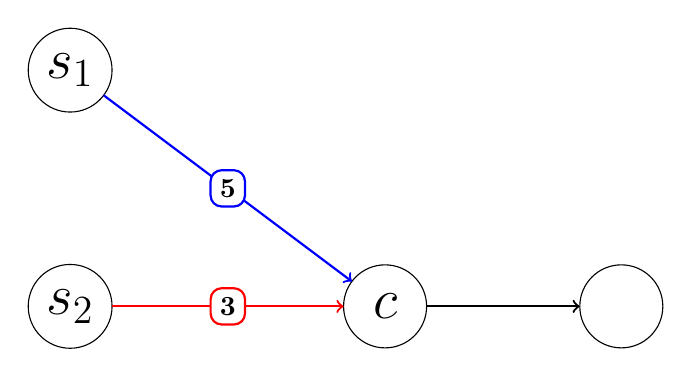
\begin{tikzpicture}
  \SetGraphUnit{5}
    \tikzset{
  EdgeStyle/.append style = {->} }
   \tikzstyle{VertexStyle}=[shape = circle, draw, minimum size = 30pt]
   \renewcommand{\VertexLightFillColor}{orange}
  \Vertex[x=0,y=3, L = {\huge $s_2$}]{a3};

  \Vertex[x=0,y=6, L = {\huge $s_1$}]{a1}


  \Vertex[x=4,y=3, L = {\huge $c$}]{c}

 \SetVertexNoLabel
\Vertex[x=7,y=3]{d}

      \Edge(c)(d)
  \tikzset{
  EdgeStyle/.append style = {blue} }
  \Edge[label = 5](a1)(c)   
 
  
    \tikzset{
  EdgeStyle/.append style = {red} }
    \Edge[label = 3](a3)(c)
  


\end{tikzpicture}
}
\end{center}

\end{frame}
 \begin{frame}{Model: The communication process}
 Example for $P=13$ and $\tau = 3$.
\begin{center}
\scalebox{0.6}{

\begin{tikzpicture}
  \SetGraphUnit{5}
    \tikzset{
  EdgeStyle/.append style = {->} }
   \tikzstyle{VertexStyle}=[shape = circle, draw, minimum size = 30pt]
   \renewcommand{\VertexLightFillColor}{orange}
  \Vertex[x=0,y=3, L = {\huge $s_2$}]{a3};

  \Vertex[x=0,y=6, L = {\huge $s_1$}]{a1}


  \Vertex[x=4,y=3, L = {\huge $c$}]{c}
   \draw[red] (4,3) circle (6ex);
 \SetVertexNoLabel
\Vertex[x=7,y=3]{d}

      \Edge(c)(d)
  \tikzset{
  EdgeStyle/.append style = {blue} }
  \Edge[label = 5](a1)(c)   
 
  
    \tikzset{
  EdgeStyle/.append style = {red} }
    \Edge[label = 3](a3)(c)
  
      
       \node (0) at (5,1){\includegraphics[scale=0.2]{col1.png}};


\end{tikzpicture}
}
\end{center}
\begin{definition}

There is a \textcolor{blue}{collision} between two routes when their messages go through the first vertex of a common arc at the same time.
\end{definition}

\pause
\centering
 \textcolor{red}{Periodicity must be taken into consideration.}
 \includegraphics[scale=0.1]{cols1.png} 


\end{frame}



 \begin{frame}{Assignment}

 Example for $P=13$ and $\tau = 3$.
 
\begin{center}
 \begin{multicols}{2}
\scalebox{0.6}{

\begin{tikzpicture}
  \SetGraphUnit{5}
    \tikzset{
  EdgeStyle/.append style = {->} }
   \tikzstyle{VertexStyle}=[shape = circle, draw, minimum size = 30pt]
   \renewcommand{\VertexLightFillColor}{orange}
  \Vertex[x=0,y=3, L = {\huge $s_2$}]{a3};

  \Vertex[x=0,y=6, L = {\huge $s_1$}]{a1}


  \Vertex[x=4,y=3, L = {\huge $c$}]{c}
  
 \SetVertexNoLabel
\Vertex[x=7,y=3]{d}

      \Edge(c)(d)

    
  \tikzset{
  EdgeStyle/.append style = {blue} }
  \Edge[label = 5](a1)(c)   
 
  
    \tikzset{
  EdgeStyle/.append style = {red} }
    \Edge[label = 3](a3)(c)
  \node (0) at (0,2.2){0};
      \node (0) at (0,5.2){0};
       \node (0) at (5,2){\includegraphics[scale=0.2]{col1.png}};


\end{tikzpicture}
}
\pause
\hspace{0.2cm}$\rightarrow$
\scalebox{0.6}{

\begin{tikzpicture}
  \SetGraphUnit{5}
    \tikzset{
  EdgeStyle/.append style = {->} }
   \tikzstyle{VertexStyle}=[shape = circle, draw, minimum size = 30pt]
   \renewcommand{\VertexLightFillColor}{orange}
  \Vertex[x=0,y=3, L = {\huge $s_2$}]{a3};

  \Vertex[x=0,y=6, L = {\huge $s_1$}]{a1}


  \Vertex[x=4,y=3, L = {\huge $c$}]{c}
  
 \SetVertexNoLabel
\Vertex[x=7,y=3]{d}

      \Edge(c)(d)

    
  \tikzset{
  EdgeStyle/.append style = {blue} }
  \Edge[label = 5](a1)(c)   
 
  
    \tikzset{
  EdgeStyle/.append style = {red} }
    \Edge[label = 3](a3)(c)
    \node (0) at (0,2.2){0};
      \node (0) at (0,5.2){1};
       \node (0) at (5,2){\includegraphics[scale=0.2]{col2.png}};


\end{tikzpicture}
}
\end{multicols}
\end{center}

\vspace{1cm}
\begin{center}
Choosing the offset such that there is no collisions.
\end{center}
\begin{definition}
An \textcolor{blue}{Assignment} is a choice of offset for each message.
\end{definition}
\end{frame}

\begin{frame}{A first problem}
\only<1>{
 \begin{center}

\scalebox{0.35}{

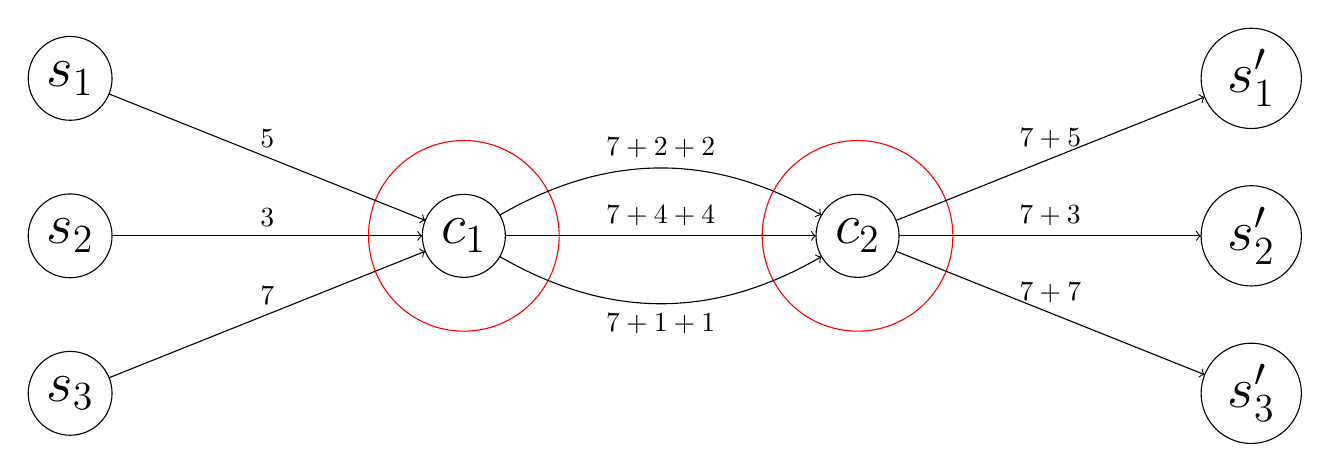
\begin{tikzpicture}
  \SetGraphUnit{5}
    \tikzset{
  EdgeStyle/.append style = {->} }
   \tikzstyle{VertexStyle}=[shape = circle, draw, minimum size = 30pt]
   \renewcommand{\VertexLightFillColor}{orange}
  \Vertex[x=0,y=4, L = {\huge $s_1$}]{s1};
  \Vertex[x=0,y=2, L = {\huge $s_2$}]{s2};
\Vertex[x=0,y=0, L = {\huge $s_3$}]{s3};
\Vertex[x=15,y=4, L = {\huge $s_1'$}]{s1p};
\Vertex[x=15,y=2, L = {\huge $s_2'$}]{s2p};
\Vertex[x=15,y=0, L = {\huge $s_3'$}]{s3p};
\draw[red] (10,2) circle (8ex);
\draw[red] (5,2) circle (8ex);
\Vertex[x=10,y=2, L = {\huge $c_2$}]{c2};

  \Vertex[x=5,y=2, L = {\huge $c_1$}]{c1}
  
 %\SetVertexNoLabel
  %\Vertex[x=4,y=2]{n1}

  %\Edge[label = $5$](s1)(c1)
  %\Edge[label = $7 + 4+4$](c1)(c2)
  %\Edge[label = $3$](s2)(c1)
   %\Edge[label = $7$](s3)(c1)
  %  \Edge[label = $7+3$](c2)(s2p)
 %  \Edge[label = $7+7$](c2)(s3p)
%\Edge[label = $7 + 5$](c2)(s1p)
\path (s1) edge [->] node[anchor=south]{$5$} (c1);

\path (s2) edge [->] node[anchor=south]{$3$} (c1);
\path (s3) edge [->] node[anchor=south]{$7$} (c1);
\path (c2) edge [->] node[anchor=south]{$7+3$} (s2p);
\path (c2) edge [->] node[anchor=south]{$7+7$} (s3p);

\path (c2) edge [->] node[anchor=south]{$7+5$} (s1p);

\path (c1) edge [->] node[anchor=south]{$7+4+4$} (c2);

\path (c1) edge [->,bend left=30] node[anchor=south]{$7+2+2$} (c2);
\path (c1) edge [->,bend right=30] node[anchor=north]{$7+1+1$} (c2);

  %\draw[->,line width=0.5pt] (5,2.51) parabola bend (7.5,3.5) (10,2.51);
 %\draw[->,line width=0.5pt] (5,1.49) parabola bend (7.5,0.5) (10,1.49);
 

\end{tikzpicture}
}
\end{center}
}
\only<2->{
   \begin{center}
\scalebox{0.35}{

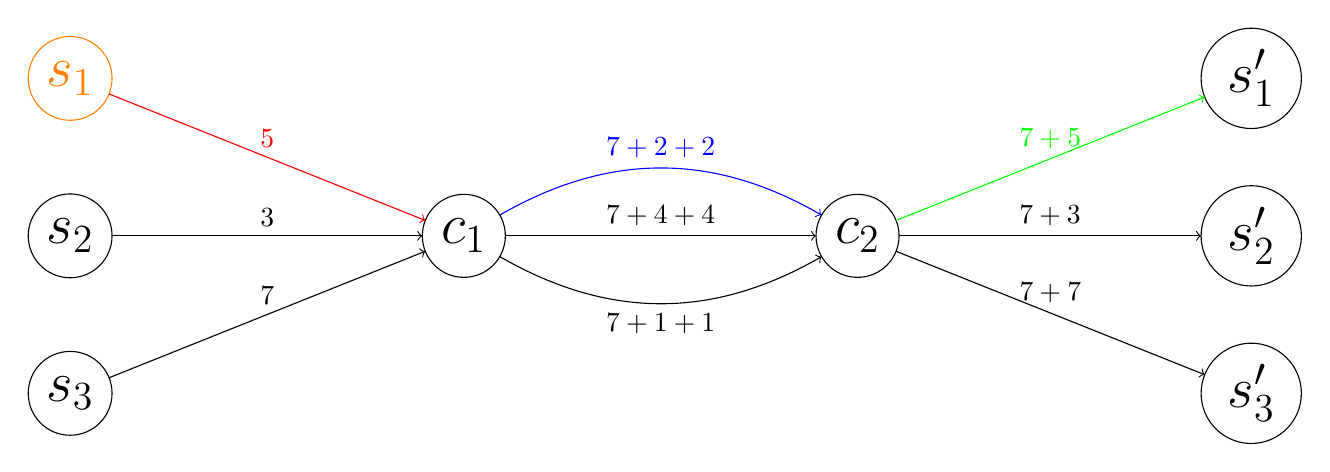
\begin{tikzpicture}
  \SetGraphUnit{5}
    \tikzset{
  EdgeStyle/.append style = {->} }
   \tikzstyle{VertexStyle}=[shape = circle, draw, minimum size = 30pt,orange]
     \Vertex[x=0,y=4, L = {\huge $s_1$}]{s1};


   \tikzstyle{VertexStyle}=[shape = circle, draw, minimum size = 30pt,black]

  \Vertex[x=0,y=2, L = {\huge $s_2$}]{s2};
\Vertex[x=0,y=0, L = {\huge $s_3$}]{s3};
\Vertex[x=15,y=4, L = {\huge $s_1'$}]{s1p};
\Vertex[x=15,y=2, L = {\huge $s_2'$}]{s2p};
\Vertex[x=15,y=0, L = {\huge $s_3'$}]{s3p};

\Vertex[x=10,y=2, L = {\huge $c_2$}]{c2};
  \Vertex[x=5,y=2, L = {\huge $c_1$}]{c1}

 %\SetVertexNoLabel
  %\Vertex[x=4,y=2]{n1}

  %\Edge[label = $5$](s1)(c1)
  %\Edge[label = $7 + 4+4$](c1)(c2)
  %\Edge[label = $3$](s2)(c1)
   %\Edge[label = $7$](s3)(c1)
  %  \Edge[label = $7+3$](c2)(s2p)
 %  \Edge[label = $7+7$](c2)(s3p)
%\Edge[label = $7 + 5$](c2)(s1p)
\path (s1) edge [red,->] node[anchor=south]{$5$} (c1);

\path (s2) edge [->] node[anchor=south]{$3$} (c1);
\path (s3) edge [->] node[anchor=south]{$7$} (c1);
\path (c2) edge [->] node[anchor=south]{$7+3$} (s2p);
\path (c2) edge [->] node[anchor=south]{$7+7$} (s3p);

\path (c2) edge [green,->] node[anchor=south]{$7+5$} (s1p);

\path (c1) edge [->] node[anchor=south]{$7+4+4$} (c2);

\path (c1) edge [blue,->,bend left=30] node[anchor=south]{$7+2+2$} (c2);
\path (c1) edge [->,bend right=30] node[anchor=north]{$7+1+1$} (c2);

  %\draw[->,line width=0.5pt] (5,2.51) parabola bend (7.5,3.5) (10,2.51);
 %\draw[->,line width=0.5pt] (5,1.49) parabola bend (7.5,0.5) (10,1.49);
 

\end{tikzpicture}
}

\pause
\vspace{0.5cm}
\includegraphics[width=0.7\textwidth]{time0.pdf}

\end{center}

}
\pause
 \begin{exampleblock}{Periodic Assignment for Zero Latency (PAZL)}
  Given a routed network, find an assignment such that there is no collisions in $c_1$ and $c_2$.
 \end{exampleblock}
\end{frame}



\begin{frame}{Complexity}
\begin{theorem}\label{th:hardness_contention_depth}
PAZL is $\NP$-complete.
\end{theorem}

    \scalebox{0.5}{
    \begin{tikzpicture}
    \tikzset{
      LabelStyle/.style = { rectangle, rounded corners, draw,
        font = \bfseries },
    EdgeStyle/.append style = {->} }
      \SetGraphUnit{5}
      
  

      \tikzstyle{VertexStyle}=[shape = circle, draw, minimum size = 20pt]
  \tikzset{
   VertexStyle/.append style = { thick, loosely dashdotted} }
  \Vertex[x=-8,y=3]{u}
        \tikzset{
      VertexStyle/.append style = {dashed, thick} }
    \Vertex[x=-7,y=5]{v}

      \tikzset{
      VertexStyle/.append style = {dotted, thick} }
    \Vertex[x=-6,y=4]{w}

       
    
  \tikzset{
       EdgeStyle/.append style = {black,solid,-} }

       \Edge(u)(v)
       \Edge(u)(w)
     \node (1) at (-3,4){\Huge $\rightarrow$};
      
     \node (2) at (-7,0){\Huge H};

     \end{tikzpicture}
     }

     Reduction of an instance H of vertex-coloring to an instance of PAZL. 
\end{frame}

\begin{frame}{Complexity}
\begin{theorem}\label{th:hardness_contention_depth}
PAZL is $\NP$-complete.
\end{theorem}

    \scalebox{0.5}{
    \begin{tikzpicture}
    \tikzset{
      LabelStyle/.style = { rectangle, rounded corners, draw,
        font = \bfseries },
    EdgeStyle/.append style = {->} }
      \SetGraphUnit{5}
      
       \onslide<3->{
      \node[draw,dotted, thick,circle] (s3) at (4, 2) {$w^1$}; 
      }
      \onslide<2->{
      \node[draw,dashed, thick,circle] (s2) at (0, 4) {$v^1$}; 
      }
      \node[draw,circle,thick, loosely dashdotted] (s1) at (0, 6) {$u^1$}; 
 \onslide<3->{
      \node[draw,dotted, thick,circle] (t3) at (12, 3) {$w^2$}; 
      }
       \onslide<2->{
      \node[draw,dashed, thick,circle] (t2) at (10, 5) {$v^2$}; 
      }
      \node[draw,circle,thick, loosely dashdotted] (t1) at (10, 1) {$u^2$}; 
      

      \tikzstyle{VertexStyle}=[shape = circle, draw, minimum size = 20pt]
  \tikzset{
   VertexStyle/.append style = {thick, loosely dashdotted} }
  \Vertex[x=-8,y=3]{u}
        \tikzset{
      VertexStyle/.append style = {dashed, thick} }
    \Vertex[x=-7,y=5]{v}

      \tikzset{
      VertexStyle/.append style = {dotted, thick} }
    \Vertex[x=-6,y=4]{w}
    \tikzset{
      VertexStyle/.append style = {black,solid} }
      
       
       \SetVertexNoLabel
       \onslide<2->{
       \Vertex[x=2,y=5]{A}}

       \onslide<3->{
       \Vertex[x=6,y=3]{E}}

       \tikzset{
       EdgeStyle/.append style = {dashed, thick} }
       \onslide<2->{
       \Edge(s2)(A)
       
      \Edge(A)(t2)
      }
 
       
       \tikzset{
      EdgeStyle/.append style = {dotted, thick} }
      \onslide<3->{
       \Edge(s3)(E)
       \Edge(E)(t3)
       } 
  \tikzset{
       EdgeStyle/.append style = {thick, loosely dashdotted} }
      \onslide<1>{\Edge(s1)(t1)}
       \onslide<2->{
       \Edge(s1)(A)
      
      }
      \onslide<2>
      { \Edge(A)(t1)}
      \onslide<3->{
       \Edge(A)(E)
              
       \Edge(E)(t1)
       }
       
  \tikzset{
       EdgeStyle/.append style = {black,-,solid} }

       \Edge(u)(v)
       \Edge(u)(w)
     \node (1) at (-3,4){\Huge $\rightarrow$};
      
     \node (2) at (-7,0){\Huge H};
      \node (3) at (10,0){\Huge N};
     \end{tikzpicture}
     }

     Reduction of an instance H of vertex-coloring to an instance of PAZL. 
\end{frame}


\begin{frame}{Complexity}
\begin{theorem}\label{th:hardness_contention_depth}
PAZL is $\NP$-complete.
\end{theorem}

    \scalebox{0.5}{
    \begin{tikzpicture}
    \tikzset{
      LabelStyle/.style = { rectangle, rounded corners, draw,
        font = \bfseries },
    EdgeStyle/.append style = {->} }
      \SetGraphUnit{5}
      
      
      \node[draw,circle] (s3) at (4, 2) {$w^1$}; 
      \node[draw,circle] (s2) at (0, 4) {$v^1$}; 
      \node[draw,circle] (s1) at (0, 6) {$u^1$}; 

      \node[draw,circle] (t3) at (12, 3) {$w^2$}; 
      \node[draw,circle] (t2) at (10, 5) {$v^2$}; 
      \node[draw,circle] (t1) at (10, 2) {$u^2$}; 
      

      \tikzstyle{VertexStyle}=[shape = circle, draw, minimum size = 20pt]
  \tikzset{
   VertexStyle/.append style = {blue} }
  \Vertex[x=-8,y=3]{u}
        \tikzset{
      VertexStyle/.append style = {green} }
    \Vertex[x=-7,y=5]{v}

      \tikzset{
      VertexStyle/.append style = {red} }
    \Vertex[x=-6,y=4]{w}
    \tikzset{
      VertexStyle/.append style = {black} }
      
       
       \SetVertexNoLabel
       \Vertex[x=2,y=5]{A}


       \Vertex[x=6,y=3]{E}

       \tikzset{
       EdgeStyle/.append style = {green} }
       \Edge(s2)(A)
       
      \Edge(A)(t2)
 
       
       \tikzset{
      EdgeStyle/.append style = {red} }
       \Edge(s3)(E)
       \Edge(E)(t3) 
  \tikzset{
       EdgeStyle/.append style = {blue} }
       \Edge(s1)(A)
    
       \Edge(A)(E)
              
       \Edge(E)(t1)
       
  \tikzset{
       EdgeStyle/.append style = {black,-} }

       \Edge(u)(v)
       \Edge(u)(w)
     \node (1) at (-3,4){\Huge $\rightarrow$};
      
     \node (2) at (-7,0){\Huge H};
      \node (3) at (10,0){\Huge N};
     \end{tikzpicture}
     }

     Reduction of an instance H of vertex-coloring to an instance of PAZL. A P-coloration of H is equivalent to a P-periodic Assignment of N.
\end{frame}

\begin{frame}{Solving PAZL}
Algorithms to solve PAZL:
\begin{itemize}
  \item Exsitence of a solution for moderate loads using polynomial time algorithms.
  \item FPT Algorithm with the number of routes as parameter.
  \end{itemize}
\begin{center}
  \includegraphics[scale=0.4]{pazlshort8.pdf}\\
 \end{center} 


\end{frame}



\begin{frame}{Assignment}
 
 \begin{center}
\scalebox{0.3}{

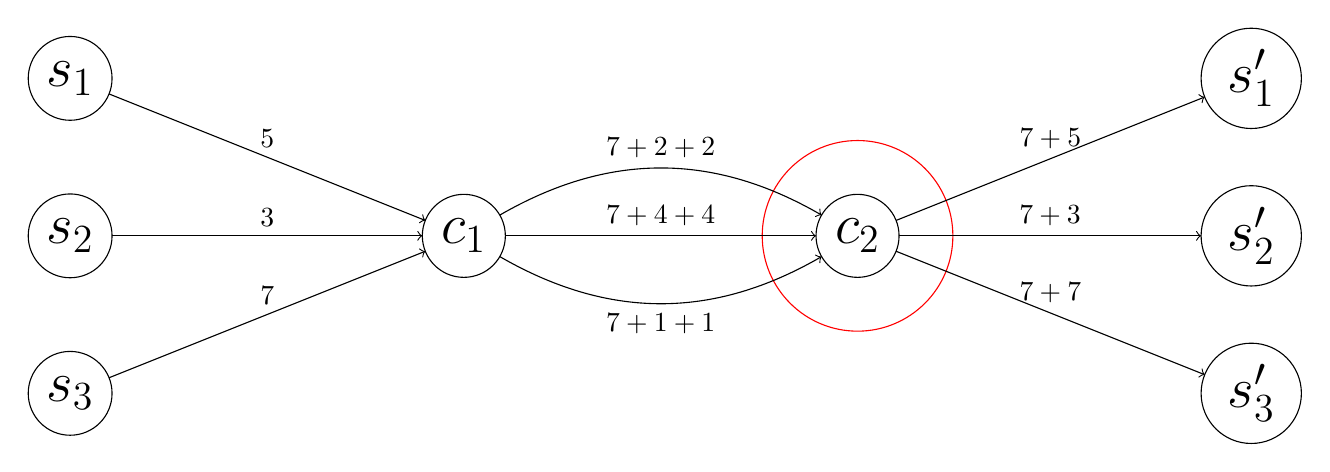
\begin{tikzpicture}
  \SetGraphUnit{5}
    \tikzset{
  EdgeStyle/.append style = {->} }
   \tikzstyle{VertexStyle}=[shape = circle, draw, minimum size = 30pt]
   \renewcommand{\VertexLightFillColor}{orange}
  \Vertex[x=0,y=4, L = {\huge $s_1$}]{s1};
  \Vertex[x=0,y=2, L = {\huge $s_2$}]{s2};
\Vertex[x=0,y=0, L = {\huge $s_3$}]{s3};
\Vertex[x=15,y=4, L = {\huge $s_1'$}]{s1p};
\Vertex[x=15,y=2, L = {\huge $s_2'$}]{s2p};
\Vertex[x=15,y=0, L = {\huge $s_3'$}]{s3p};
\draw[red] (10,2) circle (8ex);
\Vertex[x=10,y=2, L = {\huge $c_2$}]{c2};

  \Vertex[x=5,y=2, L = {\huge $c_1$}]{c1}
  
 %\SetVertexNoLabel
  %\Vertex[x=4,y=2]{n1}

  %\Edge[label = $5$](s1)(c1)
  %\Edge[label = $7 + 4+4$](c1)(c2)
  %\Edge[label = $3$](s2)(c1)
   %\Edge[label = $7$](s3)(c1)
  %  \Edge[label = $7+3$](c2)(s2p)
 %  \Edge[label = $7+7$](c2)(s3p)
%\Edge[label = $7 + 5$](c2)(s1p)
\path (s1) edge [->] node[anchor=south]{$5$} (c1);

\path (s2) edge [->] node[anchor=south]{$3$} (c1);
\path (s3) edge [->] node[anchor=south]{$7$} (c1);
\path (c2) edge [->] node[anchor=south]{$7+3$} (s2p);
\path (c2) edge [->] node[anchor=south]{$7+7$} (s3p);

\path (c2) edge [->] node[anchor=south]{$7+5$} (s1p);

\path (c1) edge [->] node[anchor=south]{$7+4+4$} (c2);

\path (c1) edge [->,bend left=30] node[anchor=south]{$7+2+2$} (c2);
\path (c1) edge [->,bend right=30] node[anchor=north]{$7+1+1$} (c2);

  %\draw[->,line width=0.5pt] (5,2.51) parabola bend (7.5,3.5) (10,2.51);
 %\draw[->,line width=0.5pt] (5,1.49) parabola bend (7.5,0.5) (10,1.49);
 

\end{tikzpicture}
}
\end{center}


\pause


In $c_2$, one can choose the \textcolor{blue}{waiting time} before sending back the answer.\\

\begin{center}
  \includegraphics[scale=0.6]{BBU}\\
 \end{center} 


\pause 
\begin{definition}
Redefinition of the notion of \textcolor{blue}{assignment}: a choice of offsets and waiting times for each route without collisions.
\end{definition}
   
\end{frame}
\begin{frame}{Transmission Time}

 \begin{center}
\scalebox{0.35}{

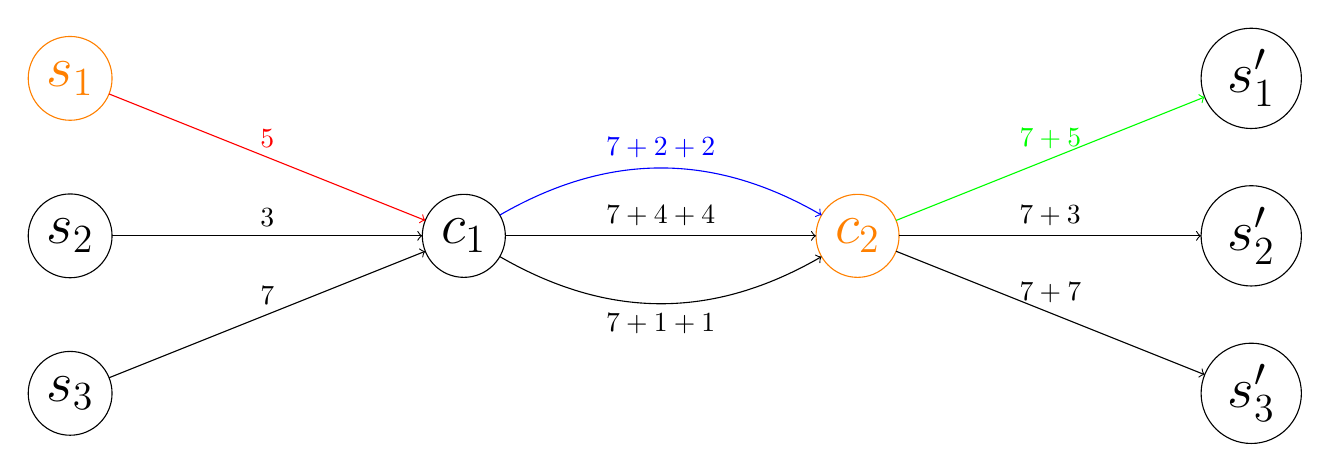
\begin{tikzpicture}
  \SetGraphUnit{5}
    \tikzset{
  EdgeStyle/.append style = {->} }
   \tikzstyle{VertexStyle}=[shape = circle, draw, minimum size = 30pt,orange]
     \Vertex[x=0,y=4, L = {\huge $s_1$}]{s1};

\Vertex[x=10,y=2, L = {\huge $c_2$}]{c2};

   \tikzstyle{VertexStyle}=[shape = circle, draw, minimum size = 30pt,black]

  \Vertex[x=0,y=2, L = {\huge $s_2$}]{s2};
\Vertex[x=0,y=0, L = {\huge $s_3$}]{s3};
\Vertex[x=15,y=4, L = {\huge $s_1'$}]{s1p};
\Vertex[x=15,y=2, L = {\huge $s_2'$}]{s2p};
\Vertex[x=15,y=0, L = {\huge $s_3'$}]{s3p};

  \Vertex[x=5,y=2, L = {\huge $c_1$}]{c1}

 %\SetVertexNoLabel
  %\Vertex[x=4,y=2]{n1}

  %\Edge[label = $5$](s1)(c1)
  %\Edge[label = $7 + 4+4$](c1)(c2)
  %\Edge[label = $3$](s2)(c1)
   %\Edge[label = $7$](s3)(c1)
  %  \Edge[label = $7+3$](c2)(s2p)
 %  \Edge[label = $7+7$](c2)(s3p)
%\Edge[label = $7 + 5$](c2)(s1p)
\path (s1) edge [red,->] node[anchor=south]{$5$} (c1);

\path (s2) edge [->] node[anchor=south]{$3$} (c1);
\path (s3) edge [->] node[anchor=south]{$7$} (c1);
\path (c2) edge [->] node[anchor=south]{$7+3$} (s2p);
\path (c2) edge [->] node[anchor=south]{$7+7$} (s3p);

\path (c2) edge [green,->] node[anchor=south]{$7+5$} (s1p);

\path (c1) edge [->] node[anchor=south]{$7+4+4$} (c2);

\path (c1) edge [blue,->,bend left=30] node[anchor=south]{$7+2+2$} (c2);
\path (c1) edge [->,bend right=30] node[anchor=north]{$7+1+1$} (c2);

  %\draw[->,line width=0.5pt] (5,2.51) parabola bend (7.5,3.5) (10,2.51);
 %\draw[->,line width=0.5pt] (5,1.49) parabola bend (7.5,0.5) (10,1.49);
 

\end{tikzpicture}
}

\vspace{1cm}
\includegraphics[width=0.7\textwidth]{time.pdf}

\end{center}



\end{frame}
\begin{frame}{Deadline and Problem}

Each route must have a transmission time lower or equal to a given \textbf{deadline}.
\pause
\vspace{1cm}

 \begin{exampleblock}{Periodic Assignment for Low Latency (PALL)}
  Given a routed network, find an assignment such that the deadline constraint is satisfied for each route.
 \end{exampleblock}

\vspace{1cm}
\pause
 PALL is NP-complete.

\end{frame}

\section{Solving PALL on simple topologies}


\subsection{A two stage approach for PALL}
\begin{frame}{A two stage approach for PALL}

\textbf{First step:} We fix the offset of the route such that there is no collisions in $c_1$.
\begin{center}
\scalebox{0.4}{

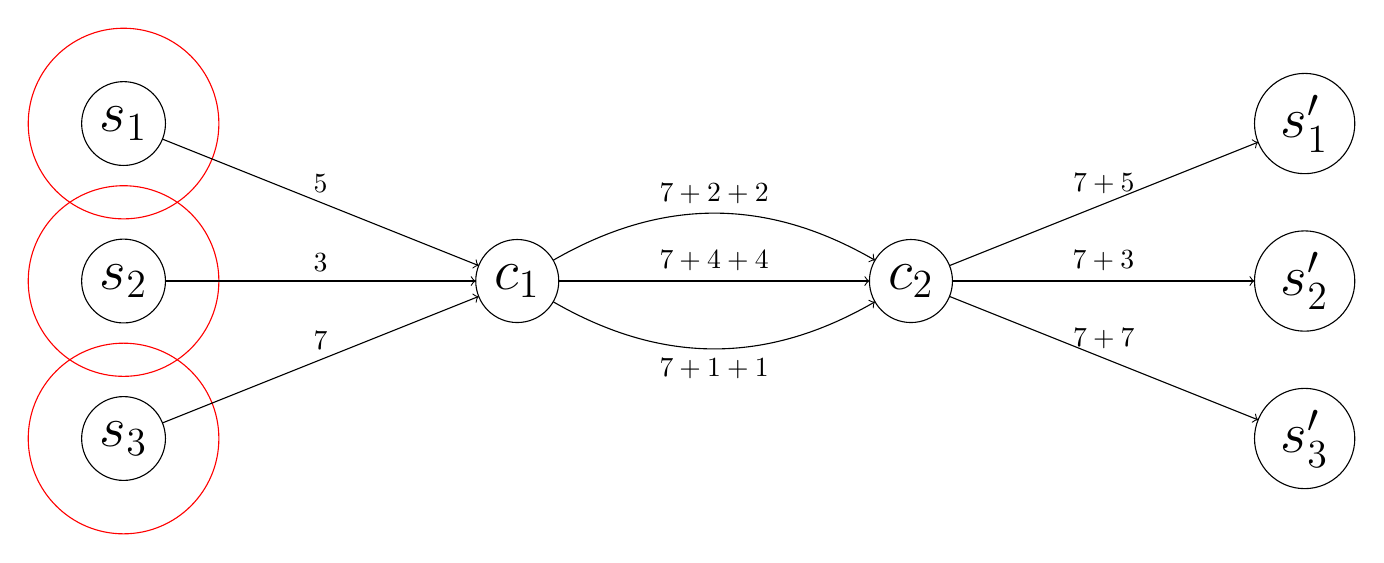
\begin{tikzpicture}
  \SetGraphUnit{5}
    \tikzset{
  EdgeStyle/.append style = {->} }
   \tikzstyle{VertexStyle}=[shape = circle, draw, minimum size = 30pt]
   \renewcommand{\VertexLightFillColor}{orange}
  \Vertex[x=0,y=4, L = {\huge $s_1$}]{s1};
  \Vertex[x=0,y=2, L = {\huge $s_2$}]{s2};
\Vertex[x=0,y=0, L = {\huge $s_3$}]{s3};
\Vertex[x=15,y=4, L = {\huge $s_1'$}]{s1p};
\Vertex[x=15,y=2, L = {\huge $s_2'$}]{s2p};
\Vertex[x=15,y=0, L = {\huge $s_3'$}]{s3p};
\Vertex[x=10,y=2, L = {\huge $c_2$}]{c2};
\draw[red] (0,0) circle (8ex);
\draw[red] (0,2) circle (8ex);
\draw[red] (0,4) circle (8ex);
  \Vertex[x=5,y=2, L = {\huge $c_1$}]{c1}
  
 %\SetVertexNoLabel
  %\Vertex[x=4,y=2]{n1}

  %\Edge[label = $5$](s1)(c1)
  %\Edge[label = $7 + 4+4$](c1)(c2)
  %\Edge[label = $3$](s2)(c1)
   %\Edge[label = $7$](s3)(c1)
  %  \Edge[label = $7+3$](c2)(s2p)
 %  \Edge[label = $7+7$](c2)(s3p)
%\Edge[label = $7 + 5$](c2)(s1p)
\path (s1) edge [->] node[anchor=south]{$5$} (c1);

\path (s2) edge [->] node[anchor=south]{$3$} (c1);
\path (s3) edge [->] node[anchor=south]{$7$} (c1);
\path (c2) edge [->] node[anchor=south]{$7+3$} (s2p);
\path (c2) edge [->] node[anchor=south]{$7+7$} (s3p);

\path (c2) edge [->] node[anchor=south]{$7+5$} (s1p);

\path (c1) edge [->] node[anchor=south]{$7+4+4$} (c2);

\path (c1) edge [->,bend left=30] node[anchor=south]{$7+2+2$} (c2);
\path (c1) edge [->,bend right=30] node[anchor=north]{$7+1+1$} (c2);

  %\draw[->,line width=0.5pt] (5,2.51) parabola bend (7.5,3.5) (10,2.51);
 %\draw[->,line width=0.5pt] (5,1.49) parabola bend (7.5,0.5) (10,1.49);
 

\end{tikzpicture}
}
 \end{center}
 \pause
\textbf{Second Step:}
 \begin{exampleblock}{Waiting Time Assignment (WTA)}
 Given the routed network and the offsets for all routes, find an assignment satisfying the deadlines constraints.
 \end{exampleblock}

\begin{center}
 \scalebox{0.4}{


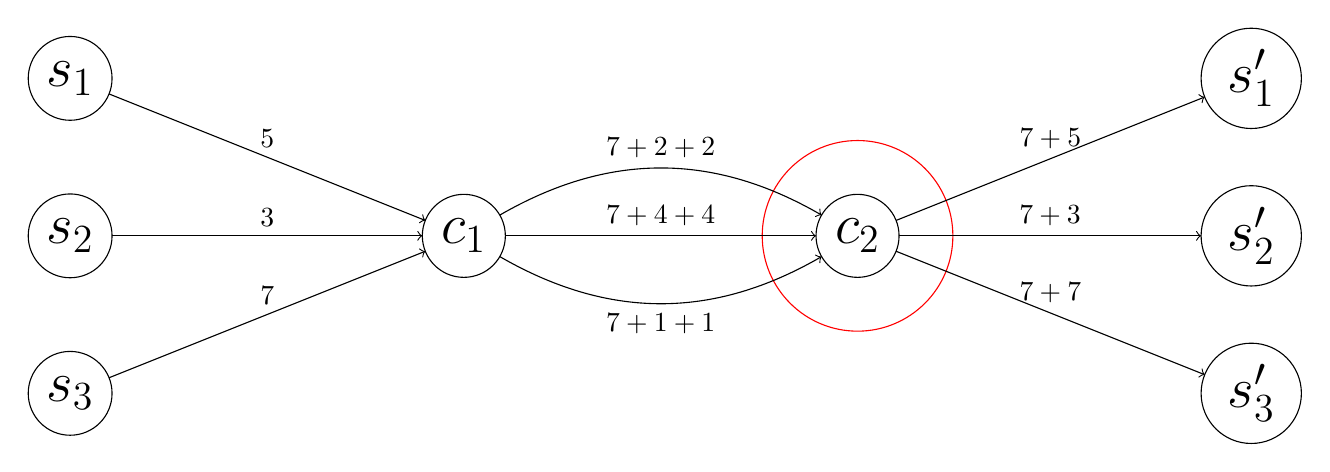
\begin{tikzpicture}
  \SetGraphUnit{5}
    \tikzset{
  EdgeStyle/.append style = {->} }
   \tikzstyle{VertexStyle}=[shape = circle, draw, minimum size = 30pt]
   \renewcommand{\VertexLightFillColor}{orange}
  \Vertex[x=0,y=4, L = {\huge $s_1$}]{s1};
  \Vertex[x=0,y=2, L = {\huge $s_2$}]{s2};
\Vertex[x=0,y=0, L = {\huge $s_3$}]{s3};
\Vertex[x=15,y=4, L = {\huge $s_1'$}]{s1p};
\Vertex[x=15,y=2, L = {\huge $s_2'$}]{s2p};
\Vertex[x=15,y=0, L = {\huge $s_3'$}]{s3p};
\Vertex[x=10,y=2, L = {\huge $c_2$}]{c2};

  \Vertex[x=5,y=2, L = {\huge $c_1$}]{c1}
  \draw[red] (10,2) circle (8ex);
 %\SetVertexNoLabel
  %\Vertex[x=4,y=2]{n1}

  %\Edge[label = $5$](s1)(c1)
  %\Edge[label = $7 + 4+4$](c1)(c2)
  %\Edge[label = $3$](s2)(c1)
   %\Edge[label = $7$](s3)(c1)
  %  \Edge[label = $7+3$](c2)(s2p)
 %  \Edge[label = $7+7$](c2)(s3p)
%\Edge[label = $7 + 5$](c2)(s1p)
\path (s1) edge [->] node[anchor=south]{$5$} (c1);

\path (s2) edge [->] node[anchor=south]{$3$} (c1);
\path (s3) edge [->] node[anchor=south]{$7$} (c1);
\path (c2) edge [->] node[anchor=south]{$7+3$} (s2p);
\path (c2) edge [->] node[anchor=south]{$7+7$} (s3p);

\path (c2) edge [->] node[anchor=south]{$7+5$} (s1p);

\path (c1) edge [->] node[anchor=south]{$7+4+4$} (c2);

\path (c1) edge [->,bend left=30] node[anchor=south]{$7+2+2$} (c2);
\path (c1) edge [->,bend right=30] node[anchor=north]{$7+1+1$} (c2);

  %\draw[->,line width=0.5pt] (5,2.51) parabola bend (7.5,3.5) (10,2.51);
 %\draw[->,line width=0.5pt] (5,1.49) parabola bend (7.5,0.5) (10,1.49);
 

\end{tikzpicture}
}
\end{center}
\end{frame}

\begin{frame}{Solving WTA: A greedy algorithm}

          \begin{center}
   \begin{tabularx}{0.7\textwidth}{|c|X|X|X|X|X|X|}
    \hline
     Route& \textcolor{blue}{$0$}  & \only<1-4>{ $1$ }\only<5->{\textcolor{red}{$1$}}& \only<1-2>{ $2$ }\only<3->{\textcolor{green}{$2$}}& $3$ & $4$\\
    \hline
    Deadline & $10$ &$15$&\only<1-2>{ $5$ }\only<3-4>{\textbf{5}}\only<5->{ $5$ }&$7$&$32$\\
    \hline
     Arrival time in $c_2$ & $0$ &$2$&$3$&$16$&$17$\\
    \hline
    Waiting time & \only<2->{$0$} &\only<6->{$6$}&\only<4->{$1$}&\only<8->{$0$}&\only<10->{$15$}\\
    \hline
      \end{tabularx}

\vspace{1cm}
      
       A run of GreedyDeadline with $P = 20, \tau = 4$.

      \includegraphics[width=0.7\textwidth]{step1.pdf}
\pause
\pause
\includegraphics[width=0.7\textwidth]{ste2.pdf}
\pause
\pause
\includegraphics[width=0.7\textwidth]{step3.pdf}
\pause
\pause
\includegraphics[width=0.7\textwidth]{step4.pdf}
\pause
\pause
\includegraphics[width=0.7\textwidth]{step5.pdf}

 
      \end{center}
\end{frame}


\begin{frame}{Solving WTA: Polynomial time algorithms}

  
   \textbf{MLS:}  Polynomial time algorithm. Finds a solution minimizing the date at which all messages are scheduled. 
   \pause
   \textcolor{red}{Periodicity not managed.}      


   \pause 
 

   \includegraphics[width=0.54\textwidth]{pmls.pdf}
\pause

  \textbf{PMLS:} 
\includegraphics[width=0.9\textwidth]{pmls2.pdf}

 \pause

   \textbf{ASPMLS:} FPT-Algorithm based on PMLS $\rightarrow$ Always find a solution if existing.

\end{frame}



\subsection{Results}
\begin{frame}{Results: Algorithms for WTA}
\centering
\includegraphics[width=0.9\textwidth]{retour_210002.pdf}

\end{frame}
\begin{frame}{Results: PMLS against statistical multiplexing}
\centering
\includegraphics[width=\textwidth]{stochastic2.pdf}
\end{frame}



\begin{frame}{Mixing C-RAN traffic with Best-Effort Traffic}
\textbf{C-RAN traffic}: High priority, deterministic traffic, scheduled with minimal latency.

\vspace{0.5cm}

\pause
\textbf{Best Effort traffic}: Low priority, stochastic law on arrivals, no specific rules on forwarding.

\vspace{0.5cm}

\pause
PMLS creates long sequences of C-RAN traffic in which there is no free spaces for BE traffic.

\vspace{1cm}
\pause
\centering
\includegraphics[width=0.9\textwidth]{space.pdf}

\end{frame}


\begin{frame}{Mixing C-RAN traffic with Best-Effort Traffic}
\centering
\includegraphics[width=0.9\textwidth]{res.pdf}

\end{frame}


\section{Synchronized PALL}
\subsection{Definition of SPALL}



\begin{frame}{Synchronized Version of PALL}
\begin{center}
\scalebox{0.4}{

\begin{tikzpicture}
  \SetGraphUnit{5}
    \tikzset{
  EdgeStyle/.append style = {->} }
   \tikzstyle{VertexStyle}=[shape = circle, draw, minimum size = 30pt]
   \renewcommand{\VertexLightFillColor}{orange}
  \Vertex[x=0,y=4, L = {\huge $s_1$}]{s1};
  \Vertex[x=0,y=2, L = {\huge $s_2$}]{s2};
\Vertex[x=0,y=0, L = {\huge $s_3$}]{s3};
\Vertex[x=15,y=4, L = {\huge $s_1'$}]{s1p};
\Vertex[x=15,y=2, L = {\huge $s_2'$}]{s2p};
\Vertex[x=15,y=0, L = {\huge $s_3'$}]{s3p};
\Vertex[x=10,y=2, L = {\huge $c_2$}]{c2};

  \Vertex[x=5,y=2, L = {\huge $c_1$}]{c1}
  
 %\SetVertexNoLabel
  %\Vertex[x=4,y=2]{n1}

  %\Edge[label = $5$](s1)(c1)
  %\Edge[label = $7 + 4+4$](c1)(c2)
  %\Edge[label = $3$](s2)(c1)
   %\Edge[label = $7$](s3)(c1)
  %  \Edge[label = $7+3$](c2)(s2p)
 %  \Edge[label = $7+7$](c2)(s3p)
%\Edge[label = $7 + 5$](c2)(s1p)
\path (s1) edge [->] node[anchor=south]{$5$} (c1);

\path (s2) edge [->] node[anchor=south]{$3$} (c1);
\path (s3) edge [->] node[anchor=south]{$7$} (c1);
\path (c2) edge [->] node[anchor=south]{$7+3$} (s2p);
\path (c2) edge [->] node[anchor=south]{$7+7$} (s3p);

\path (c2) edge [->] node[anchor=south]{$7+5$} (s1p);

\path (c1) edge [->] node[anchor=south]{$7+4+4$} (c2);

\path (c1) edge [->,bend left=30] node[anchor=south]{$7+2+2$} (c2);
\path (c1) edge [->,bend right=30] node[anchor=north]{$7+1+1$} (c2);

  %\draw[->,line width=0.5pt] (5,2.51) parabola bend (7.5,3.5) (10,2.51);
 %\draw[->,line width=0.5pt] (5,1.49) parabola bend (7.5,0.5) (10,1.49);
 
\only<1>\draw[red] (0,0) circle (8ex);
\only<1>\draw[red] (0,2) circle (8ex);
\only<1>\draw[red] (0,4) circle (8ex);
\only<2->\draw[red] (5,2) circle (8ex);
\only<2->\draw[red] (10,2) circle (8ex);
\end{tikzpicture}
}
 
\end{center}
The antennas are \textbf{synchronized}: All messages are emited at the same date.

\pause
There is no more offsets, but a buffer in each contention point.

\pause
\begin{definition}
An \textcolor{blue}{Assignment} is a choice of buffering time for each message in every contention point.
\end{definition}
\pause
 \begin{exampleblock}{Synchronized Periodic Assignment for Low Latency (SPALL)}
 Given the routed network, find an assignment satisfying the deadlines constraints.
 \end{exampleblock}
\end{frame}
\begin{frame}{Transmission Time in SPALL}

\begin{center}
\scalebox{0.3}{

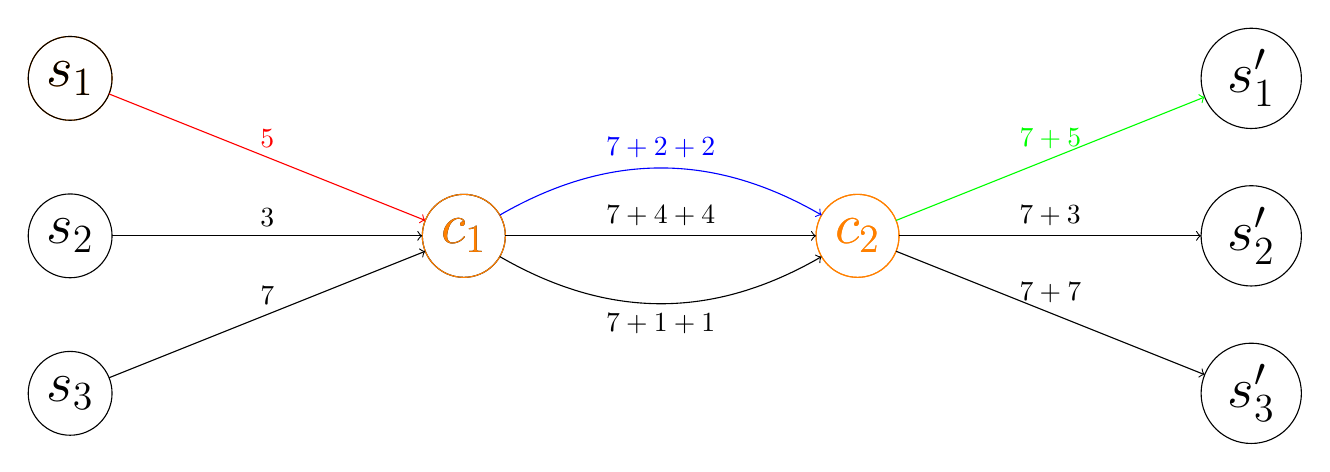
\begin{tikzpicture}
  \SetGraphUnit{5}
    \tikzset{
  EdgeStyle/.append style = {->} }
  \onslide<1>{
   \tikzstyle{VertexStyle}=[shape = circle, draw, minimum size = 30pt,orange]
     \Vertex[x=0,y=4, L = {\huge $s_1$}]{s1};

\Vertex[x=10,y=2, L = {\huge $c_2$}]{c2};
   \tikzstyle{VertexStyle}=[shape = circle, draw, minimum size = 30pt,black]
\Vertex[x=5,y=2, L = {\huge $c_1$}]{c1}
  }
   \onslide<2->{
   \tikzstyle{VertexStyle}=[shape = circle, draw, minimum size = 30pt,orange]
      \Vertex[x=5,y=2, L = {\huge $c_1$}]{c1}

\Vertex[x=10,y=2, L = {\huge $c_2$}]{c2};
   \tikzstyle{VertexStyle}=[shape = circle, draw, minimum size = 30pt,black]
 \Vertex[x=0,y=4, L = {\huge $s_1$}]{s1};
  }


   \tikzstyle{VertexStyle}=[shape = circle, draw, minimum size = 30pt,black]

  \Vertex[x=0,y=2, L = {\huge $s_2$}]{s2};
\Vertex[x=0,y=0, L = {\huge $s_3$}]{s3};
\Vertex[x=15,y=4, L = {\huge $s_1'$}]{s1p};
\Vertex[x=15,y=2, L = {\huge $s_2'$}]{s2p};
\Vertex[x=15,y=0, L = {\huge $s_3'$}]{s3p};



 %\SetVertexNoLabel
  %\Vertex[x=4,y=2]{n1}

  %\Edge[label = $5$](s1)(c1)
  %\Edge[label = $7 + 4+4$](c1)(c2)
  %\Edge[label = $3$](s2)(c1)
   %\Edge[label = $7$](s3)(c1)
  %  \Edge[label = $7+3$](c2)(s2p)
 %  \Edge[label = $7+7$](c2)(s3p)
%\Edge[label = $7 + 5$](c2)(s1p)
\path (s1) edge [red,->] node[anchor=south]{$5$} (c1);

\path (s2) edge [->] node[anchor=south]{$3$} (c1);
\path (s3) edge [->] node[anchor=south]{$7$} (c1);
\path (c2) edge [->] node[anchor=south]{$7+3$} (s2p);
\path (c2) edge [->] node[anchor=south]{$7+7$} (s3p);

\path (c2) edge [green,->] node[anchor=south]{$7+5$} (s1p);

\path (c1) edge [->] node[anchor=south]{$7+4+4$} (c2);

\path (c1) edge [blue,->,bend left=30] node[anchor=south]{$7+2+2$} (c2);
\path (c1) edge [->,bend right=30] node[anchor=north]{$7+1+1$} (c2);

  %\draw[->,line width=0.5pt] (5,2.51) parabola bend (7.5,3.5) (10,2.51);
 %\draw[->,line width=0.5pt] (5,1.49) parabola bend (7.5,0.5) (10,1.49);
 

\end{tikzpicture}
}

\end{center}
 \begin{overprint}

\onslide<1>\includegraphics[width=\textwidth]{time.pdf}
\onslide<2>\includegraphics[width=\textwidth]{time2.pdf}

\end{overprint}

\end{frame}
\begin{frame}{Deeper networks}
\centering
%\includegraphics[width=0.9\textwidth]{graphmodel.pdf}
\scalebox{0.4}{

\begin{tikzpicture}
  \SetGraphUnit{5}
    \tikzset{
  EdgeStyle/.append style = {->} }
   \tikzstyle{VertexStyle}=[shape = circle, draw, minimum size = 30pt]
 

  \node (s8) at (0,10.5) {\includegraphics[width = 1cm]{rrh.png}};
  \node (s7) at (0,9) {\includegraphics[width = 1cm]{rrh.png}};
  \node (s6) at (0,7.5) {\includegraphics[width = 1cm]{rrh.png}};
  \node (s5) at (0,6) {\includegraphics[width = 1cm]{rrh.png}};
  \node (s4) at (0,4.5) {\includegraphics[width = 1cm]{rrh.png}};
  \node (s3) at (0,3) {\includegraphics[width = 1cm]{rrh.png}};
  \node (s2) at (0,1.5) {\includegraphics[width = 1cm]{rrh.png}};
  \node (s1) at (0,0) {\includegraphics[width = 1cm]{rrh.png}};
  
   \node (b2) at (10,7.25) {\includegraphics[width = 1cm]{bbu.png}};
   \node (b1) at (10,2.25) {\includegraphics[width = 1cm]{bbu.png}};

   \node (t6) at (8,7.25) {\includegraphics[width = 1cm]{switch.png}};
   \node (t5) at (8,2.25) {\includegraphics[width = 1cm]{switch.png}};
   \node (t4) at (4,9.75) {\includegraphics[width = 1cm]{switch.png}};
   \node (t3) at (4,6.75) {\includegraphics[width = 1cm]{switch.png}};
   \node (t2) at (4,3.75) {\includegraphics[width = 1cm]{switch.png}};
   \node (t1) at (4,0.75) {\includegraphics[width = 1cm]{switch.png}};

\path (s1) edge [<->,blue]  (t1);
\path (s2) edge [<->,green]  (t1);
\path (s3) edge [<->,red]  (t2);
\path (s4) edge [<->,orange]  (t2);
\path (s5) edge [<->,brown]  (t3);
\path (s6) edge [<->,purple]  (t3);
\path (s7) edge [<->,pink]  (t4);
\path (s8) edge [<->]  (t4);

\path (t1) edge [<->,blue]  (t5);
\path (t1) edge [<->,green]  (t6);
\path (t2) edge [<->,red]  (t5);
\path (t2) edge [<->,orange]  (t6);
\path (t3) edge [<->,brown]  (t5);
\path (t3) edge [<->,purple]  (t6);
\path (t4) edge [<->,pink]  (t5);
\path (t4) edge [<->]  (t6);

\path (t6) edge [<->,thick]  (b2);
\path (t5) edge [<->,thick]  (b1);


\node (k8) at (30,10.5) {$t_8$};
\node (k7) at (30,9) {$t_7$};
\node (k6) at (30,7.5) {$t_6$};
\node (k5) at (30,6) {$t_5$};
\node (k4) at (30,4.5) {$t_4$};
\node (k3) at (30,3) {$t_3$};
\node (k2) at (30,1.5) {$t_2$};
\node (k1) at (30,0) {$t_1$};

  \node (s8) at (14,10.5) {$s_8$};
  \node (s7) at (14,9) {$s_7$};
  \node (s6) at (14,7.5) {$s_6$};
  \node (s5) at (14,6) {$s_5$};
  \node (s4) at (14,4.5) {$s_4$};
  \node (s3) at (14,3) {$s_3$};
  \node (s2) at (14,1.5) {$s_2$};
  \node (s1) at (14,0) {$s_1$};


  
  \node (t10) at (26,9.75) {$c_{10}$};
   \node (t9) at (26,6.75) {$c_9$};
   \node (t8) at (26,3.75) {$c_8$};
   \node (t7) at (26,0.75) {$c_7$};
   \node (t6) at (22,7.25) {$c_6$};
   \node (t5) at (22,2.25) {$c_5$};
   \node (t4) at (18,9.75) {$c_4$};
   \node (t3) at (18,6.75) {$c_3$};
   \node (t2) at (18,3.75) {$c_2$};
   \node (t1) at (18,0.75) {$c_1$};

\path (s1) edge [->,blue]  (t1);
\path (s2) edge [->,green]  (t1);
\path (s3) edge [->,red]  (t2);
\path (s4) edge [->,orange]  (t2);
\path (s5) edge [->,brown]  (t3);
\path (s6) edge [->,purple]  (t3);
\path (s7) edge [->,pink]  (t4);
\path (s8) edge [->]  (t4);

\path (t1) edge [->,blue]  (t5);
\path (t1) edge [->,green]  (t6);
\path (t2) edge [->,red]  (t5);
\path (t2) edge [->,orange]  (t6);
\path (t3) edge [->,brown]  (t5);
\path (t3) edge [->,purple]  (t6);
\path (t4) edge [->,pink]  (t5);
\path (t4) edge [->]  (t6);

\path (k1) edge [<-,blue]  (t7);
\path (k2) edge [<-,green]  (t7);
\path (k3) edge [<-,red]  (t8);
\path (k4) edge [<-,orange]  (t8);
\path (k5) edge [<-,brown]  (t9);
\path (k6) edge [<-,purple]  (t9);
\path (k7) edge [<-,pink]  (t10);
\path (k8) edge [<-]  (t10);

\path (t7) edge [<-,blue]  (t5);
\path (t7) edge [<-,green]  (t6);
\path (t8) edge [<-,red]  (t5);
\path (t8) edge [<-,orange]  (t6);
\path (t9) edge [<-,brown]  (t5);
\path (t9) edge [<-,purple]  (t6);
\path (t10) edge [<-,pink]  (t5);
\path (t10) edge [<-]  (t6);




\end{tikzpicture}
}

Each contention point at the same level can be solved independantly.

Once all the contention points of the same level have been solved, we deal with the contention points of the next level.

\end{frame}

\subsection{Solving SPALL: Compact representation}
\begin{frame}{Compact representation}
A compact representation of an assignment on a contention point $u$ is a pair ($O_u$,\only<1>{...}\only<2->{$S_u$}).

	\includegraphics[width=0.65\linewidth]{order}
  \pause
  \includegraphics[width=\linewidth]{subset}


\pause
\begin{itemize}
  \item Not all assignments have a compact representation.
  \pause
  \item Several assignments can have the same compact representation.
  \end{itemize}
\end{frame}
\begin{frame}{Solving SPALL: Assignment from a compact representation }
Inductive construction of an assignment from the compact representation. 

Example for $((2,1,0,3),\{1\})$ on a single contention point .


	\includegraphics[width=0.5\linewidth]{compacttoassignment1}
\pause
\includegraphics[width=0.5\linewidth]{compacttoassignment2}
\pause
\includegraphics[width=0.5\linewidth]{compacttoassignment3}
\pause
\includegraphics[width=0.5\linewidth]{compacttoassignment4}
\pause

\begin{itemize}
  \item The assignment built from a compact representation is \textcolor{red}{minimal}.
  \pause

  \item Help to reduce the number of solutions to explore. Exponential in the number of routes an depth of the network.
  \end{itemize}
\end{frame}
\subsection{Solving SPALL: Local search algorithms }
\begin{frame}{Neighborhood and Local Search Algorithms}

 Neighborood of a compact representation defined by a permutation:
\begin{center}
\scalebox{0.7}{

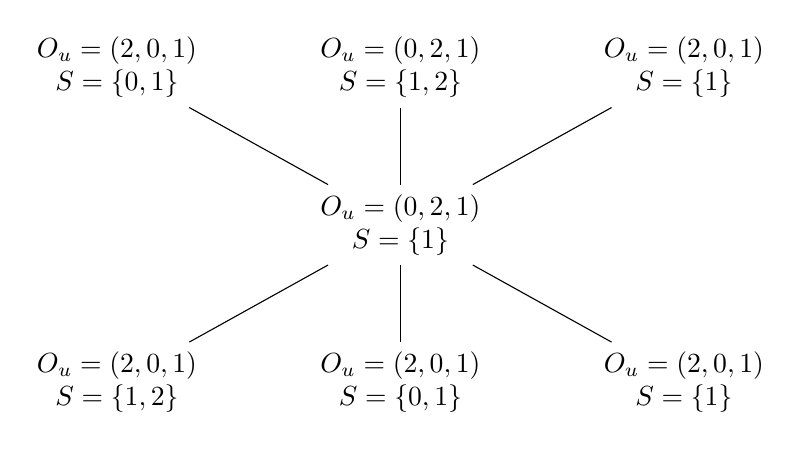
\begin{tikzpicture}
  \SetGraphUnit{5}
    \tikzset{
  EdgeStyle/.append style = {->} }
   \tikzstyle{VertexStyle}=[shape = circle, draw, minimum size = 50pt]
 

  \node[align=center] (p0) at (10,5) {$O_u = (0,2,1)$\\$S = \{1\}$};
  \node[align=center] (p1) at (10,7) {$O_u = (0,2,1)$\\$S = \{1,2\}$};
  \node[align=center] (p2) at (13.6,7) {$O_u = (2,0,1)$\\$S = \{1\}$};
  \node[align=center] (p3) at (13.6,3) {$O_u = (2,0,1)$\\$S = \{1\}$};
  \node[align=center] (p4) at (10,3) {$O_u = (2,0,1)$\\$S = \{0,1\}$};
  \node[align=center] (p5) at (6.4,3) {$O_u = (2,0,1)$\\$S = \{1,2\}$};
  \node[align=center] (p6) at (6.4,7) {$O_u = (2,0,1)$\\$S = \{0,1\}$};


 
\path (p0) edge [-] (p1);
\path (p0) edge [-] (p2);
\path (p0) edge [-] (p3);
\path (p0) edge [-] (p4);
\path (p0) edge [-] (p5);
\path (p0) edge [-] (p6);



\end{tikzpicture}
}

\end{center}

\pause

Initial Solution : Greedy similar to PALL.
\pause

   \textbf{Algorithms :} Hill Climbing ,
   \pause
   Tabu Search, 
\pause Simulated Annealing, 
\pause Branch and Bound.


\end{frame}

\subsection{Results}
\begin{frame}{Results: Algorithms to solve SPALL}
\begin{center}
	\includegraphics[width=\linewidth]{all8routes}

\end{center}
\end{frame}
\section{Conclusion}
\begin{frame}{Conclusion}


\begin{block}{Key result.}
  Deterministic Networking is the best way to manage deterministic flows.
\end{block}

\begin{block}{Industrial prototype in development.}
\begin{itemize}
    \item Hot topic in telecommunications.
    \item 2 registered patents.
      \end{itemize}
\end{block}
  
\begin{block}{Complexification of the model.}
  \begin{itemize}
      \item Different bandwidth.
      \item Not the same period for all messages.
      \item Different messages size.
    \end{itemize}
\end{block}

\begin{block}{Open Questions.}
  \begin{itemize}
      \item Complexity of PALL on star networks.
      \item Performances of PALL algorithms on deeper networks.
    \end{itemize}
\end{block}


\end{frame}

\begin{frame}
\begin{center}
\huge{\scshape Thank You \\ For your time and attention !}
\end{center}
\vspace{1cm}

 \begin{multicols}{2}
Published Papers:
\begin{itemize}
  \item 
\tiny{Dominique Barth, Maël Guiraud, Brice Leclerc, Olivier Marcé, Yann Strozecki\\
Deterministic Scheduling of Periodic Messages for Cloud RAN. ICT 2018: 405-410}
  \item \tiny{Dominique Barth, Maël Guiraud, Yann Strozecki\\
Deterministic Contention Management for Low Latency Cloud RAN over an Optical Ring. ONDM 2019: 479-491}
\end{itemize}

Pre-print:
\begin{itemize}
  \item \tiny{Dominique Barth, Maël Guiraud, Brice Leclerc, Olivier Marcé, Yann Strozecki\\
Deterministic Scheduling of Periodic Messages for Cloud RAN (2021, long version). Submitted to Networks.}
  \item \tiny{Maël Guiraud, Yann Strozecki\\
Scheduling periodic messages on a shared link (2021). Submitted to MFCS.}
\end{itemize}

\end{multicols}

\end{frame}




\end{document}
